\documentclass[12pt]{article} 
\usepackage[utf8]{inputenc}
\usepackage{geometry}
\geometry{letterpaper}
\usepackage{graphicx} 
\usepackage{parskip}
\usepackage{booktabs}
\usepackage{array} 
\usepackage{paralist} 
\usepackage{verbatim}
\usepackage{subfig}
\usepackage{fancyhdr}
\usepackage{sectsty}

\pagestyle{fancy}
\renewcommand{\headrulewidth}{0pt} 
\lhead{}\chead{}\rhead{}
\lfoot{}\cfoot{\thepage}\rfoot{}


%%% ToC (table of contents) APPEARANCE
\usepackage[nottoc,notlof,notlot]{tocbibind} 
\usepackage[titles,subfigure]{tocloft}
\renewcommand{\cftsecfont}{\rmfamily\mdseries\upshape}
\renewcommand{\cftsecpagefont}{\rmfamily\mdseries\upshape} %

\usepackage{amsmath}
\usepackage{amssymb}
\usepackage{empheq}
\usepackage{xcolor}
\usepackage{bbm}
\renewcommand{\L}[1]{\mathcal{L}\{#1\}}
\newcommand{\ans}[1]{\boxed{\text{#1}}}
\newcommand{\vecs}[1]{\langle #1\rangle}
\renewcommand{\hat}[1]{\widehat{#1}}
\newcommand{\F}[1]{\mathcal{F}(#1)}
\renewcommand{\P}{\mathbb{P}}
\newcommand{\R}{\mathbb{R}}
\newcommand{\qed}{\quad \blacksquare}
\newcommand{\brak}[1]{\left\langle #1 \right\rangle}
\newcommand{\C}{\mathbb{C}}
\newcommand{\bra}[1]{\left\langle #1 \right\vert }
\newcommand{\ket}[1]{\left\vert #1 \right\rangle}
\newcommand{\E}{\mathbb{E}}
\newcommand{\ind}{\mathbbm{1}}
\newcommand{\abs}[1]{\left\vert #1 \right\vert}

\usepackage{tikz}
\usepackage{pgfplots}
\pgfplotsset{compat=1.18}

\title{APMA 1930W: Probabilities in Quantum Mechanics}
\author{Milan Capoor}
\date{Fall 2023}

\begin{document}
\maketitle
\section*{Lecture 1: Sept 6}
Outline of the course:
\begin{enumerate}
    \item A single particle
    \begin{itemize}
        \item Probabilities
        \item Waves
    \end{itemize}

    \item Entanglement (multiple particles)
    \item Applications and consequences
    \begin{itemize}
        \item Bell's theorem
        \item Teleportation
        \item Free will (Conway-Kochen theorem)
        \item Encryption
        \item Quantum computing 
    \end{itemize}
\end{enumerate}

\section*{Lecture 2: Sept 8}
\subsection*{The 2-Slit Experiment}
\textbf{A wave:} we can imagine a 1-color wave at a single frequency
\[A\cos(\omega t - kx + \phi)\]
where 
\begin{itemize}
    \item $\omega$ is the frequency (rad/s) which describes the speed of vertical oscillation
    \item $k$ is rad/m which describes speed of horizontal movement
    \item $\phi$ is the phase shift 
    \item $A$ is the amplitude 
\end{itemize}

(the goal of the $kx$ term is to grow proportionally with the $\omega t$ term to create a constant value without oscillation to send through the detector)

This wave can be decomposed:
\[A\cos(\omega t - kx + \phi) = A\cos \phi \cos(\omega t - kx) - A\sin \phi \sin(\omega t - kx)\]

\emph{Proof:}

Using Euler's identity, $e^{iz} = \cos z + i\sin z$, 
\begin{align*}
    \Re(A \cos(\omega t - kx + \phi)) &= \Re(A e^{i(\omega t - kx + \phi)})\\
    &= \Re(Ae^{i \phi} (\cos(\omega t - kx) + i\sin (\omega t - kx)))\\
    &= \Re(A(\cos \phi + i \sin \phi) (\cos(\omega t - kx) + i\sin (\omega t - kx)))\\
    &=  A\cos \phi \cos(\omega t - kx) - A\sin \phi \sin(\omega t - kx)
\end{align*}

\textbf{The Experiment:}
We imagine a variable with two narrow slits bombarded by the wave $\tilde A \cos(\omega t - kx)$.

Our goal is to find the equation of the wave impacting a detector at $x=1$ after the diffusion effect of the variable. Because there are two slits, the waves ($\psi_1, \psi_2$) from each slit will interfere (linear sum) to create a new wave on the detector at a specific point $\psi(x, y, t)$ after traveling a distance $r_1$ or $r_2$ respectively. Thus,
\[\psi(x, y, t) = \psi_1(x, y, t) + \psi(x, y, t) = A_1 \cos(\omega t - k r_1) + A_2(\cos(\omega t - k r_2))\]
where $A_1 = \tilde A/\sqrt{r_1}$ and $A_2 = \tilde A/\sqrt{r_2}$ to take into account fading intensity over time.

All of this together will give us the amplitude of composite waves at the point on the screen which we square to get the intensity ($I \propto A^2$)

Calculated across the entire screen this will give a distribution of intensities which \textbf{perfectly} matches the distribution of collision locations of single-particles over a long period of time. 

\section*{Lecture 3: Sept 11}
\subsection*{Stern-Gerlach Experiment}
We set up two non-symmetric magnets on top of each other with North pole facing South pole and a gap between them. We send an electron through and it will either go up or down to land on two specific points on the detector, indicating that each electron has a magnetic moment of exactly $\hbar/2$ or $-\hbar/2$.

Important findings:
\begin{enumerate}
    \item This happens for ANY orientation of the machine
    \item The result is definite. If we put a second S-G device at the detector point, ALL the particles that went up the first time will also go up the second time (and the same for down). That is,
    
    \[\P(\lambda_n(t + 1) = 1 | \lambda_n(t) = 1) = 1, \quad \P(\lambda_n(t + 1)=  1 | \lambda_n(t) = -1) = 0\]
    where $\lambda_n$ is the state of the particle after going through the device ($\lambda_n : t \mapsto \{-1, 1\}$)
\end{enumerate}

If we now send the particle through a new ``m-machine'' characterized by a new orientation $n, m \in \R_1^3 = \{v \in \R^3 : |v| = 1\} = S^2$, then the corresponding probabilities for a particle prepared in the $n$-direction is 
\begin{align*}
    \P(\lambda_m(t + 1) = 1 | \lambda_n(t) = 1) = \frac{1 + m \cdot n}{2}\\
    \P(\lambda_m(t + 1) = 1 | \lambda_n(t) = 1) = \frac{1 - m \cdot n}{2}
\end{align*}

Now we create a new experiment. A stream of N $\lambda_x = 1$ particles go through an orthogonal $z$-detector such that $\P(\lambda_z = 1) = N/2$ and $\P(\lambda_z = -1) = N/2$. If we magnetically bend these two back through the same $x$-detector so the input is 1/2 $\lambda_z = 1$ and 1/2 $\lambda_z = -1$, we still see $\P(\lambda_x = 1) = N$. 

But! If we do not bend these into the same detector but place another $x$-detector after the $z$-detector we find that $\P(\lambda_x = 1 | \lambda_z = 1) = N/4$ and $\P(\lambda_x = -1 | \lambda_z = -1 ) = N/4$ -- exactly what would have happened regardless of the earlier $x$-detector

\section*{Lecture 4: Sept 13}
\textbf{Feynman's Version:}
Using three machines in series, we are able to take an input, split it, and put it back together regardless of preparation. Using the normal process, we prepare $\lambda_x = 1$ then send it through one $z$-Feynman machine with the bottom blocked (so $\P(\lambda_z = 1) = N/2$) then through a $x$-Feynman machine with the top blocked so the final output is $\P(\lambda_x = -1) = N/4$

Now we set up a new experiment: send $\lambda_x = 1$ through a $z$-Feynman machine with no block then through a $x$-Feynman machine with the top blocked. The output is $0$.

\textbf{Conclusion:} bending the streams back together is as if we never sent it through a machine at all because the particle is now in both states. 

\subsection*{Derivation of State}
\textbf{Recall the Two-slit:} we use complex variables to account for phase and model linear interference (See Lecture 2)
\[\psi(y, t) = \Re(y)e^{i\psi(y, t)} = A_1(y) e^{-ikr_1(y)} + A_2(y)e^{-ikr_2(y)}\]

In the Two-Slit Experiment the outcomes fall into $\R^2$ but in teh Stern-Gerlach Experiment, there are only two possible outcomes. 

\section*{Lecture 5: Sept 15}
\subsection*{A Complex-valued Vector Space}
(The complex-values conveniently handle phase while the vector space accounts for linear interference)

Our first task is to determine the dimensionality needed. From the experiment itself, we saw that $\R_1^3$ was sufficient to completely determine the system. Thus we do not need a higher dimensional space than $\R^3$. In mapping to the complex numbers, though, we observe that $\mathbb{C}^2$ already provides more degrees of freedom than we need. 

\textbf{Notation:}

\begin{center}
    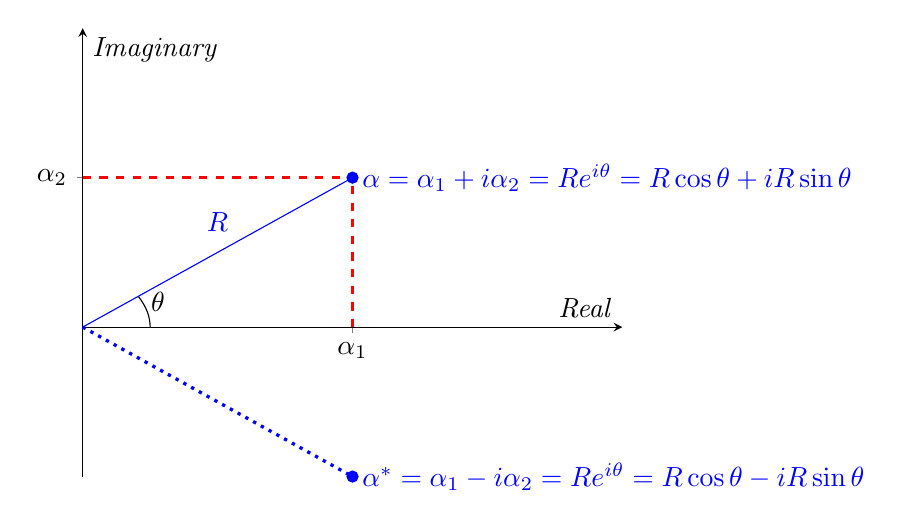
\begin{tikzpicture}
        \begin{axis}[
            axis lines=middle, 
            ylabel={\emph{Imaginary}}, 
            xlabel={\emph{Real}}, 
            xtick={1}, ytick={1},
            xticklabels={$\alpha_1$}, yticklabels={$\alpha_2$},
            xmax=2, ymax=2,
            clip=false]
            \addplot[dashed, red, very thick, domain=0:1]{1};
            \draw[dashed, red, very thick] (axis cs: 1, 0) -- (axis cs: 1, 1);
            \addplot[blue, domain=0:1]{x};
            \addplot[dotted, very thick, blue, domain=0:1]{-x};
            \draw (0.25, 0) arc (0:24:0.5) node[anchor=west, yshift=-2, xshift=1]{$\theta$};
            \filldraw[blue] (axis cs:1,1) circle (2pt) node[anchor=west]{$\alpha=\alpha_1 + i\alpha_2=Re^{i\theta} = R\cos\theta + iR\sin \theta$};
            \filldraw[blue] (axis cs:1,-1) circle (2pt) node[anchor=west]{$\alpha^*=\alpha_1 - i\alpha_2=Re^{i\theta} = R\cos\theta - iR\sin \theta$};
            \node[blue] at (axis cs: 0.5,0.7) {$R$};
        \end{axis}
    \end{tikzpicture}
\end{center}

This gives us several identities:
\[\R^2 = \alpha_1^2 + \alpha_2^2 = |\alpha|^2 = \alpha^* \alpha = (\alpha_1 - i\alpha_2)(\alpha_1 + i\alpha_2)\]

From these, we see for $a \in \mathbb{C}^2$ 
\begin{align*}
    a &= \begin{pmatrix}
        \alpha\\
        \beta
    \end{pmatrix} = \begin{pmatrix}
        \alpha_1 + i\alpha_2\\
        \beta_1 + i \beta_2
    \end{pmatrix}\\
    &\implies |a|^2 = |\alpha|^2 + |\beta|^2\\
    &= \alpha_1^2 + \alpha_2^2 + \beta_1^2 + \beta_2^2\\
    &= (\alpha^* \alpha) + (\beta^* \beta)\\
    &= \begin{pmatrix}
        \alpha_1 + i\alpha_2 & \beta_1 + i\beta_2
    \end{pmatrix}^* \begin{pmatrix}
        \alpha_1 + i\alpha_2\\
        \beta_1 + i\beta_2
    \end{pmatrix} \qquad (=a^\dagger a)\\
    &= \alpha_1^2 + \alpha_2^2 + \beta_1^2 + \beta_2^2\\
    &= \left|\begin{pmatrix}
        \alpha\\
        \beta
    \end{pmatrix}\right|^2
\end{align*}

($a^\dagger a$ is the composition of element-wise conjugate and transpose.)

\subsection*{Dirac Notation}
For $\psi \in \mathbb{C}^2$ we use $\bra{\psi}$ to designate the state of the particle corresponding to $\psi$. 

Then we define 
\[\ket{\psi} := \bra{\psi}^\dagger = \begin{pmatrix}
    \alpha\\
    \beta
\end{pmatrix}^{\dagger} = (\alpha^*, \beta^*)\]

So 
\[\brak{\psi | \psi} = \psi^\dagger \psi = |\psi|^2\]

\section*{Lecture 6: Sept 18}
\subsection*{A Better State Space}
Shortcomings of $\R_1^3$:
\begin{itemize}
    \item Nonlinear
    \item Arbitrary subset of a vector space
    \item No amplitudes
    \item Phase is difficult
\end{itemize}

\textbf{Complex Space:} $\mathbb{C} = \{\alpha_1 + i\alpha_2 | \alpha_1, \alpha_2 \in \R\}$ 

Which gives us a probability, 
\[|\alpha|^2 = \alpha_1^2 + \alpha_2^2 = \alpha^*\alpha\]

\textbf{2-Space:} $\mathbb{C}^2 = \{\begin{pmatrix}
    \alpha\\
    \beta
\end{pmatrix} : \alpha, \beta \in \C\}$

For which we introduce Dirac notation (Bra-Ket notation):
\[\ket{a} = \begin{pmatrix}
    \alpha\\\beta
\end{pmatrix}\]
so 
\[|\ket{a}|^2 = \brak{a | a} = \ket{a}^\dagger \ket{a} = \begin{pmatrix}
    \alpha^* & \beta^*
\end{pmatrix} \begin{pmatrix}
    \alpha\\
    \beta
\end{pmatrix} = |\alpha|^2 + |\beta|^2\]

\textbf{More generally:} 
\[\ket{a} = \begin{pmatrix}
    \alpha\\ \beta
\end{pmatrix}, \quad \ket{b} = \begin{pmatrix}
    \delta\\ \gamma
\end{pmatrix} \longrightarrow \brak{a | b} = \begin{pmatrix}
    \alpha\\ \beta
\end{pmatrix}^\dagger \begin{pmatrix}
    \delta\\ \gamma
\end{pmatrix} = \alpha^* \delta + \beta^* \gamma \]

We call $\brak{a | b}$ the \textbf{inner product} in $\C^2$.

\subsection*{Rules of the Inner Product}
Let $\eta_1, \eta_2 \in \C$ and $a_1, a_2, b \in \C^2$. Then
\begin{enumerate}
    \item $\brak{b | \eta_1 a_1 + \eta_2 a_2} = \eta_1 \bra{b | a_1} + \eta_2 \brak{b | a_2}$ (Linearity in Ket)
    \item $\brak{a | b}^* = \brak{b | a}$
    \item $\brak{\eta_1 a_1 + \eta_2 a_2 | b} = \eta_1^* \brak{a_1 | b} + \eta_2^* \brak{a_2 | b}$ (Conjugate linear in Bra)
\end{enumerate}

\subsection*{Moving between the two formulations}
\textbf{Recall:}
\[m, n \in \R_1^3 \implies \P(\lambda_n = 1 | \lambda_n = 1) = \frac{1+m\cdot n}{2} = \cos^2(\frac{\theta}{2})\]

\textbf{Define:}
\begin{align*}
    \ket{n^+} \in \C^2 \equiv \lambda_n = 1\\
    \ket{n^-} \in \C^2 \equiv \lambda_n = -1 \equiv \lambda_{-n} = 1
\end{align*}
So with $\ket{n^*} = \begin{pmatrix}
    \alpha\\\beta
\end{pmatrix}$, $|\alpha|^2 \propto$ probability of one outcome and $|\beta|^2 \propto$ the probability of the other outcome. 

Then we limit $\C^2$ to 
\[\C^2_1 = \{\begin{pmatrix} \alpha\\\beta \end{pmatrix}: \alpha, \beta \in \C \; | \; |\alpha|^2 + |\beta|^2 = 1\}\]

So at last we have a probability formulation 
\[|\brak{m^+ | n^+}|^2 = \frac{1 + m\cdot n}{1} = \P(\lambda_m = 1 | \lambda_n = 1) = \P(\lambda_m = 1 |\; \ket{\psi} = \ket{n^+})\]

\section*{Lecture 7: Sept 20}
\textbf{Goal:} find the mapping $n \in \R_1^3 \to \ket{n^+} \in \C_1^2$ such that 
\[\P(\lambda_m = 1 | \ket{\psi} = \ket{n^+}) = |\brak{m^+ | n^+}|^2 = \frac{1 + m\cdot n}{2}\]

\textbf{Remark:} the product $\brak{\psi | \phi}$ is often called the \emph{overlap} and is (basically) proportional to the degree of which one predicts the other 

\subsection*{The Cardinal Directions}
\begin{enumerate}
    \item Up ($\ket{u}$)
    \item Down ($\ket{d}$)
    \item Left ($\ket{l}$)
    \item Right ($\ket{r}$)
    \item In ($\ket{i}$)
    \item Out ($\ket{o}$)
\end{enumerate}

By convention and arbitrarily, we begin by choosing a coordinate system and denoting 
\[\ket{u} = \begin{pmatrix}
    1\\0
\end{pmatrix}\]

Then with $\ket{d} = \begin{pmatrix}
    \alpha\\\beta
\end{pmatrix}$, 
\begin{align*}
    \brak{u | d} &= 0 \implies \begin{pmatrix}
        1 & 0
    \end{pmatrix} \begin{pmatrix}
        \alpha\\\beta
    \end{pmatrix} = \alpha = 0\\
    \ket{d} &= \begin{pmatrix}
        0\\ \beta
    \end{pmatrix}\\
    |\beta|^2 &= 1 \implies \beta = e^{i\phi} \implies |e^{i\phi}|^2 = |e^{-i\phi}e^{i\phi}| = 1\\
    \ket{d} &= \begin{pmatrix}
        0\\e^{i\phi} 
    \end{pmatrix} = e^{i\phi} \begin{pmatrix}
        0\\1
    \end{pmatrix} \overset{\phi = 0}{=} \begin{pmatrix}
        0\\1
    \end{pmatrix}
\end{align*}
($\phi$ can be arbitrary because only the relative phase matters)

Again, we begin 
\[\ket{r} = \begin{pmatrix}
    \alpha\\\beta
\end{pmatrix}\]
From the Stern-Gerlach experiment, we know that 
\[\begin{cases}
    |\brak{u|r}|^2 = \frac{1}{2}\\
    |\brak{d|r}|^2 = \frac{1}{2} 
\end{cases} \implies \begin{cases}
    |\alpha|^2 = \frac{1}{2}\\
    |\beta|^2= \frac{1}{2}
\end{cases} \implies \begin{cases}
    \alpha = \frac{1}{\sqrt 2} e^{i\phi_1}\\
    \beta = \frac{1}{\sqrt 2} e^{i\phi_2}\\
\end{cases} \implies \ket{r} = \begin{pmatrix}
    \frac{1}{\sqrt 2} e^{i\phi_1}\\
    \frac{1}{\sqrt 2} e^{i\phi_2}
\end{pmatrix}\]
Again arbitrarily, we say $\phi_1 = \phi_2 = 0$ so 
\[\ket{r} = \begin{pmatrix}
    \frac{1}{\sqrt 2}\\
    \frac{1}{\sqrt 2}
\end{pmatrix}\]

This gives us three sets of constraints for $\ket{l} = \begin{pmatrix}
    \alpha\\\beta
\end{pmatrix}$:
\begin{align*}
    \brak{u|l} &= \begin{pmatrix}
        1 & 0
    \end{pmatrix}\begin{pmatrix}
        \alpha\\\beta
    \end{pmatrix} = \alpha\\
    \brak{d | l} = \beta\\
    \brak{r | l} = \frac{1}{\sqrt 2} \alpha + \frac{1}{\sqrt 2} \beta\\
    |\brak{u|l}|^2 = \frac{1}{2}\\
    |\brak{d|l}|^2 = \frac{1}{2}\\
    |\brak{r|l}|^2 = 0\\
\end{align*}
From all of this, 
\[\begin{cases}
    \alpha^2 = \frac{1}{2} \implies \alpha = e^{i\phi_1} \frac{1}{\sqrt 2}\\
    \beta^2 = \frac{1}{2} \implies \beta = e^{i\phi_2} \frac{1}{\sqrt 2}\\
    \frac{1}{\sqrt 2} \alpha + \frac{1}{\sqrt 2} \beta = \frac{1}{\sqrt 2}e^{i\phi_1} + \frac{1}{\sqrt 2}e^{i\phi_2} = 0 \implies e^{i\phi_1} = -e^{i\phi_2}
\end{cases}\]
so 
\[\ket{l} = \begin{pmatrix}
    \frac{1}{\sqrt 2} e^{i\phi_1}\\
    \frac{1}{\sqrt 2} e^{i\phi_2}
\end{pmatrix} = \begin{pmatrix}
    \frac{1}{\sqrt 2} e^{i\phi_1}\\
    -\frac{1}{\sqrt 2} e^{i\phi_1} 
\end{pmatrix}\]
We choose $\phi_1 = 0$ so 
\[\ket{l} = \begin{pmatrix}
    \frac{1}{\sqrt 2}
    -\frac{1}{\sqrt 2}\\
\end{pmatrix}\]

\section*{Lecture 8: Sept 22}
\subsection*{Review}
\textbf{States:}

\begin{center}
    \begin{tabular*}{5.24in}{|c|cccccc|}
        \hline
        $\R_1^3$ & $z$ & $-z$ & $x$ & $-x$ & $y$ & $-y$\\
        \hline
        &&&&&&\\
        Dirac $\C_1^2$ & $\ket{u}$ & $\ket{d}$& $\ket{r}$& $\ket{l}$& $\ket{i}$& $\ket{o}$\\
        &&&&&&\\
        Linear Alg $\C_1^2$ & $\begin{pmatrix}
            1\\0
        \end{pmatrix}$ & $\begin{pmatrix}
            0\\0
        \end{pmatrix}$& $\frac{1}{\sqrt 2}\begin{pmatrix}
            1\\1
        \end{pmatrix}$& $\frac{1}{\sqrt 2}\begin{pmatrix}
            1\\-1
        \end{pmatrix}$& $\frac{1}{\sqrt 2}\begin{pmatrix}
            1\\i
        \end{pmatrix}$& $\frac{1}{\sqrt 2}\begin{pmatrix}
            1\\-i
        \end{pmatrix}$\\
        \hline
    \end{tabular*}
\end{center}


Generically, 
\[n \in \R_1^3 \to \ket{n^+} \in \C_1^2\]
so 
\[\P(\lambda_m = 1 | \lambda_n = 1) = \P(\lambda_m = 1 | \; \ket{\psi} = \ket{n^+}) = \frac{1+ m\cdot n}{2} = \cos^2 \frac{\theta}{2} = |\brak{m^+ | n^+}|^2\]

\textbf{Remarks:}
\begin{enumerate}
    \item The representation in $\C_1^2$ is not unique. 
    \[\forall \ket{\psi} \in \C_1^2:\; e^{i\phi}\ket{\psi} = \ket{\psi}\]
\end{enumerate}

\subsection*{The Feynman Machine}
We imagine $\ket{n^+}$ through an $m$-oriented Feynman S-G machine such that the up and down states are bent back together. We can say 
\[\ket{n^+} = \brak{m^+ | n^+} \ket{m^+} + \brak{m^- | n^+}\ket{m^-}\]

\begin{center}
    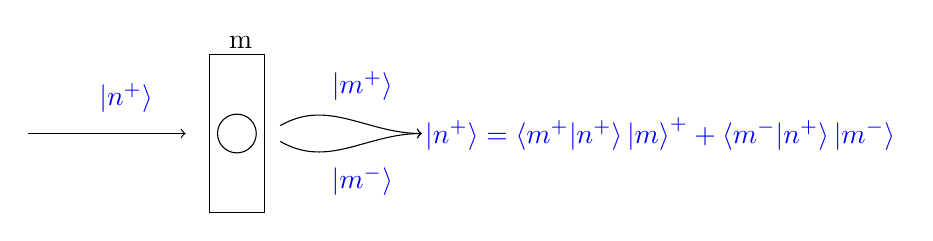
\begin{tikzpicture}
        \draw[->] (0, 0) -- (2, 0) node[yshift=3ex, xshift=-5ex, blue]{$\ket{n^+}$};
        \draw (2.3, -1) rectangle (3, 1) node[xshift=-2ex, yshift=1ex]{m};
        \draw (2.65, 0) circle (7pt);
        \draw[->] (3.2, 0.1) to [out=30, in=180]  (5, 0) node[yshift=4ex, xshift=-5ex, blue]{$\ket{m^+}$};
        \draw[->] (3.2, -0.1)  to [out=-30, in=180]  (5, 0) node[yshift=-4ex, xshift=-5ex, blue]{$\ket{m^-}$};
        \node[xshift=20ex, blue] at (5, 0) {$\ket{n^+} = \brak{m^+ | n^+} \ket m^+ + \brak{m^- | n^+}\ket{m^-}$};
    \end{tikzpicture}
\end{center}

\subsection*{Expectations}
\begin{align*}
    \E[\lambda_n |\; \ket{\psi} = \ket{m^+}] &= |\brak{n^+ | m^+}|^2 - |\brak{n^- | m^+}|^2\\
    &= \frac{1 + m\cdot n}{2} - \frac{1 - m\cdot n}{2}\\
    &= m\cdot n\\
\end{align*}

Or 
\begin{align*}
    \E[N \ind_{\lambda_n = 1} |\; \ket{\psi} = \ket{m^+}] &= N \cdot \E[\ind_{\lambda_n = 1} | \; \ket{\psi} = \ket{m^+}]\\
    &= N |\brak{m^+ | n^+}|^2
\end{align*}

\section*{Lecture 9: Sept 25}
\subsection*{Mixtures and Superposition}
By now, we have 
\[\ket r = \frac{1}{\sqrt 2} \ket u + \frac{1}{\sqrt 2} \ket d\]

We want to calculate $\E[\lambda_x | \; \ket \psi = \ket r]$

\textbf{Mixture interpretation}

We assume that because $\ket u$ and $\ket r$ are orthogonal, putting an $\ket \psi = \ket r$ prepared vector through an $x$ machine will show it go up half the time and down half the time:
\begin{align*}
    \E[\lambda_x | \; \ket \psi= \ket r] &= \frac{1}{2}\E[\lambda_x | \; \ket{\psi} = \ket{u}] + \frac{1}{2}\E[\lambda_x | \; \ket{\psi} = \ket{d}]\\
    &= \frac{1}{2}\cdot 0 + \frac{1}{2}\cdot 0\\
    &= 0
\end{align*}

But in reality, 
\[\E[\lambda_x | \; \ket \psi = \ket r] = \P(\lambda_x = 1 | \; \ket{\psi} = \ket{r}) - \P(\lambda_x = -1 | \; \ket{\psi} = \ket{r}) = 1\]

\textbf{So $\ket{r}$ is NOT a mixture of $\ket{u}$ and $\ket{d}$. It is both at the same time.}

\subsection*{Measurements}
\textbf{Hermitian Adjoint:}
\[A \in \C^{m \times n}: A^\dagger= (A')^* = (A^*)'\]

\emph{Example:}
\[A = \begin{pmatrix}
    i & 2\\
    1 + i & 1 - i\\
    3 & 2i
\end{pmatrix} \implies A^\dagger = \begin{pmatrix}
    -i & 1-i & 3\\
    2 & 1+i & -2i
\end{pmatrix}\]

\textbf{Hermitian Matrix/Operator/Transform:}
\[A \in \C^{n \times n}: A^\dagger = A\]

\emph{Example:}
\[A = \begin{pmatrix}
    3 + 2i & 1-i\\
    1 - i & 2 + i
\end{pmatrix} \implies A^\dagger = \begin{pmatrix}
    3 - 2i & 1 + i\\
    1 + i & 2-i
\end{pmatrix} \implies A \neq A^\dagger \text{ so A is not Hermitian}\]

\[A = \begin{pmatrix}
    7 & 1 + i\\
    1 - i & 8
\end{pmatrix} \implies A^\dagger = A \text{ so A is Hermitian}\]

\textbf{Spectral Theorem:}

$A \in \C^{n\times n}$ is a Hermitian matrix if and only if $A$ has the form 
\[A = \sum_{k=1}^n \lambda_k e_k e_k^\dagger = \sum_{k=1}^n \lambda_k \ket{e_k}\bra{e_k}\]
where 
\begin{itemize}
    \item $\lambda_1, \;\dots, \; \lambda_n \in \R$
    \item $e_1, \; \dots, \; e_n \in \C^n$
    \item (The vectors are orthonormal:)
    \[\brak{e_k | e_l} = e_k^\dagger e_l = \delta_{kl} = \begin{cases}
        1 \quad \text{if } k = l\\
        0 \quad \text{if } k \neq l
    \end{cases}\]
\end{itemize}
(i.e. $e_1, \; \dots, \; e_n$ are orthonormal eigenvectors with eigenvalues $\lambda_1, \;\dots, \; \lambda_n$)

\section*{Lecture 10: Sept 27}
\subsection*{Examples of the Spectral Theorem}
\textbf{Example 1:}
\[H = \begin{pmatrix}
    3 & -i\\
    i & 3
\end{pmatrix}\]

By the Spectral Theorem,
\begin{align*}
    H &= \lambda_1 e_1 e_1^\dagger + \lambda_2 e_2 e_2^\dagger\\
    &= 2\begin{pmatrix}
        \frac{1 + i}{2}\\
        \frac{1 - i}{2}
    \end{pmatrix}\begin{pmatrix}
        \frac{1 + i}{2}\\
        \frac{1 - i}{2}
    \end{pmatrix}^\dagger + 4\begin{pmatrix}
        \frac{1 + i}{2}\\
        \frac{-1 + i}{2}
    \end{pmatrix}\begin{pmatrix}
        \frac{1 + i}{2}\\
        \frac{-1 + i}{2}
    \end{pmatrix}^\dagger
\end{align*}

How do we check this? 

Answer:
\[He_1 = 2e_1 \quad He_2 = 4e_2\]
(the action of the matrix on two orthogonal vectors defines the matrix)

\subsection*{Proof of the Spectral Theorem}
\textbf{Lemma:} For a Hermitian matrix,
\[H = \sum_{k=1}^n \lambda_k e_k e_k^\dagger,\]
the values $\lambda_k \in \R$.

\emph{Proof:}

Let $\lambda$ be an eigenvalue with eigenvector $e$. Then 
\begin{align*}
    \lambda &= e^\dagger He\\
    \lambda^* = \lambda^\dagger &= (e^\dagger He)^\dagger\\
    &= e^\dagger H^\dagger e\\
    &+ e^\dagger He\\
    &= \lambda
\end{align*}
so $\lambda$ is real. 

\textbf{Remark:} the collection of eigenvalues $\lambda_k$ are called the ``spectrum''

\section*{Lecture 11: Sept 29}
\subsection*{Motivating Hermitian Operators}
Needing matrices becomes natural when we view state space as hilbert space and the matrices as linear operators on hilbert space. 

\textbf{Goal:} find an operator $o$ that maps a wave function to a particular state. 

One potential is $\ket \psi \to \ket{n^+}$ using the \textbf{projection operators:}
\[\ket{n^+}\bra{n^+}, \qquad \ket{n^-}\bra{n^-}\]

If we imagine $\sigma_n$ as a particular state, then 
\begin{align*}
    \sigma_n\ket{n^+} &= \frac{\hbar}{2}\ket{n^+}\\
    \sigma_n \ket{n^-} &= -\frac{\hbar}{2}\ket{n^-}
\end{align*}
So we note that there is a distinction between states ($\in \C_1^2$) and values (in $\R$)

Actually working it out, 
\begin{align*}
    \sigma_n := \ket{n^+}\bra{n^+} - \ket{n^-}\bra{n^-}\\
    \sigma_s \ket{n^+} &= \ket{n^+} \brak{n^+ \; | \; n^+} - \ket{n^-}\brak{n^- \; | \; n^+}\\
    &= \ket{n^+} (1) - \ket{n^-}(0) = \ket{n^+}
\end{align*}

\subsection*{Observables}
\textbf{Definition:} a Hermitian operator $\sum_i \lambda_i \ket{e_i} \bra{e_i}$ with eigenvectors corresponding to states after measurement $\ket{e_i}$ and eigenvalues $\lambda_i$ corresponding to the physical values we measure ($\{\pm \frac{\hbar}{2}\} \mapsto \{\pm 1\}$). 

This also suggests that $\big\vert \brak{e_i \; | \; \psi}
\big\vert^2$ is the probability of collapse onto a particular state $\ket{e_i}$ 

\subsection*{Computing spin states}
\begin{align*}
    \sigma_z &= \ket{z^+} \bra{z^+} - \ket{z^-}\bra{z^+}\\
    &+ \begin{pmatrix}
        1 & 0
    \end{pmatrix}\begin{pmatrix}
        1\\0 
    \end{pmatrix} - \begin{pmatrix}
        0 & 1
    \end{pmatrix} \begin{pmatrix}
        0\\1
    \end{pmatrix}\\
    &= \begin{pmatrix}
        1 & 0\\
        0 & 0
    \end{pmatrix} - \begin{pmatrix}
        0 & 0\\
        0 & 1
    \end{pmatrix}\\
    &= \begin{pmatrix}
        1 & 0\\
        0 & -1
    \end{pmatrix}
\end{align*}
Which we notice is a diagonal matrix with eigenvalues $\pm 1$. 

In the same process, 
\begin{align*}
    \ket{x^\pm} &= \frac{1}{\sqrt 2}(\ket{z^+} \pm \ket{z^-})\\
    \ket{y^\pm} &= \frac{1}{\sqrt 2}(\ket{z^+} \pm i\ket{z^-})\\
    \sigma_x &= \ket{x^+} \bra{x^+} - \ket{x^-}\bra{x^+} = \begin{pmatrix}
        0 & 1\\
        1 & 0
    \end{pmatrix}\\
    \sigma_y &= \begin{pmatrix}
        0 & -i\\
        i & 0
    \end{pmatrix}
\end{align*}

However, these matrices tell us nothing about the states or eigenvalues. To take any probabilities $\big\vert\brak{z^+ \; | \; x^+}\big\vert^2$ we would need to know the explicit form of both vectors. But! We can \emph{diagonalize} a given matrix to find the probability for any matrix. 

Taken together, these three basis matrices are the \emph{Pauli Matrices:}
\begin{empheq}[box=\fbox]{align*}
    \sigma_z &= \begin{pmatrix}
        1 & 0\\
        0 & -1
    \end{pmatrix}\\
    \sigma_x &= \begin{pmatrix}
        0 & -i\\
        i & 0
    \end{pmatrix}\\
    \sigma_y &= \begin{pmatrix}
        0 & -i\\
        i & 0
    \end{pmatrix}    
\end{empheq}

\subsection*{Expected Value}
\[A = \sum_i \lambda_i \ket{e_i} \bra{e_i}\]F
From probability theory, the expected value is just the sum of the probability times the value: 
\begin{align*}
    \E(A \; | \; \ket{\psi}) &= \sum_i \big\vert \brak{e_i \; | \; \psi} \big \vert^2 \lambda_i\\
    & = \sum_i \brak{\psi \; | \; e_i} \brak{e_i \; | \; \psi} \lambda_i\\
    &= \brak{\psi}\left(\sum_i \ket{e_i} \bra{e_i} \lambda\right)\ket{\psi}\\
    &= \brak{\psi \; | \; A \; | \;\psi}
\end{align*}

\section*{Lecture 12: Oct 2}
\subsection*{Recall}
We can represent a particular observation by the Hermitian matrix $H$:
\[H = \sum_{k=1}^n \lambda_k \ket{e_k} \bra{e_k}\]
where the vectors $e_k$ form a complete orthonormal set and $\lambda_k \in \R$. 

Then, given the starting state $\ket{\psi}$, the probability of the random result of making the observation represented by $H$, is 
\[\P(\lambda_H = \lambda_k \; | \; \ket{\psi}) = \big\vert \brak{e_k \; | \; \psi}\big \vert^2\]

This leads to the formula for expected value:
\begin{align*}
    \E[\lambda_H \; | \; \ket \psi] &= \sum_{k=1}^n \lambda_k \P(\ket{e_k})\\
    &= \sum_{k=1}^n \big\vert \brak{e_k \; | \; \psi} \big\vert^2\\
    &= \brak{\psi \; | \; H \; | \; \psi}
\end{align*}

\subsection*{Multiple measurements}
\textbf{Example:} $H_1 = \sigma_x$ and $H_2 = -\sigma_x$ with $\ket \psi = \ket r$. Then $\lambda_1 = 1$ and $\lambda_2 = -1$ (deterministically).

In general, if $H_1$ and $H_2$ share eigenvectors, then order is ``independent'':
\[\ket \psi \overunderset{H_1}{\lambda_k^1}{\longrightarrow} \ket{e_k^1} \overunderset{H_2}{\lambda_l^2}{\longrightarrow} \ket{e_l^2}\]

\textbf{Question:} When is $A = H_2 \cdot H_1$ a measurement? (i.e. when is it Hermitian?)

\emph{Answer:} If and only if $H_1$ and $H_2$ are both hermitian and share the same eigenvectors:
\begin{align*}
    H_1 &= \sum_{k=1}^n \lambda_k^1 \ket{e_k} \bra{e_k}\\
    H_2 &= \sum_{k=1}^n \lambda_k^2 \ket{e_k} \bra{e_k}
\end{align*}
(the eigenvalues can be different but the eigenvectors are the same)

\textbf{Definition:} The \emph{commutator} of $AB$ is 
\[[AB] = AB - BA\]
so $A$ and $B$ commute iff $[AB] = 0$

\section*{Lecture 13: Oct 6}

\section*{Lecture 14: Oct 11}
\textbf{The Schrodinger Equation:} Moves state forward in time deterministically based on state, environment, and time 

\subsection*{Setup}
We want a transformation $U$ that maps 
\[\begin{pmatrix}
    0\\1
\end{pmatrix} \to \begin{pmatrix}
    1\\0
\end{pmatrix} \quad \text{and} \quad \begin{pmatrix}
    1\\0
\end{pmatrix}\to \begin{pmatrix}
    0\\1
\end{pmatrix}\]

Two options are 
\begin{align*}
    \begin{pmatrix}
        0 & 1\\ 
        1 & 0
    \end{pmatrix}\begin{pmatrix}
        0\\1
    \end{pmatrix} &= \begin{pmatrix}
        1\\0
    \end{pmatrix}\\
    \begin{pmatrix}
        0 & 1\\ 
        -1 & 0
    \end{pmatrix}\begin{pmatrix}
        1\\0
    \end{pmatrix} &=   
    \begin{pmatrix}
        0\\-1
    \end{pmatrix} 
\end{align*}
Notice the second resultant is in the equivalence class of $\ket d$ with respect to phase. 

\textbf{Notation:} $\ket{\psi(t)} = U_t\ket{\psi(0)}$

\subsection*{Derivation}
\textbf{Desiderata:}
\begin{enumerate}
    \item Linearity:
    \[U_t (\ket{\psi_1(0)} + \ket{\psi_2(0)}) = U_t\ket{\psi_1(0)} + U_t\ket{\psi_2(0)} = \ket{\psi_1(t)} + \ket{\psi_2(t)}\]

    \item Conservation of Probability (i.e. $\ket{\psi(t)} \in \C_1^2$)
    \[\brak{\psi(t) \; | \; \psi(t)} = 1 \quad \forall t\]
\end{enumerate}
Already from these properties, we have a vector space and linearity so $U_t$ has a matrix representation: $U_t \in \C^{2 \times 2}$. 

Then from the second condition, be substitution,
\begin{gather*}
    \ket{\psi(t)} = U_t\ket{\psi(0)}\\ 
    \brak{\psi(t) \; | \; \psi(t)} = 1\\ 
    (U_t \ket{\psi(0)})^\dagger (U_t \ket{\psi(0)}) = 1\\
    \brak{\psi(0) U_t^\dagger U_t \; | \; \psi(0)} = 1\\
\end{gather*}
But since $(U^\dagger U)^\dagger = U^\dagger U$, we know $U^\dagger U$ is Hermitian. So we can write 
\[U_t^\dagger U_t = \sum_{i=1}^n \lambda_k \ket{e_k}\bra{e_k}\]

Plugging back in,
\begin{align*}
    \brak{\psi \bigg\vert \sum_{i=1}^n \lambda_k \ket{e_k}\bra{e_k} \bigg\vert \psi} = 1 \quad \forall \psi
\end{align*}
But as this is true \emph{for all} states, we can arbitrarily choose $\psi = e_l$ so 
\[\brak{e_l \bigg\vert \sum_{i=1}^n \lambda_k \ket{e_k}\bra{e_k} \bigg\vert e_l} = \lambda_l = 1\]

Hence, all the eigenvalues are 1. Further, $U^\dagger U = I$

\textbf{Unitary:} a matrix $U: \C_1^n \to \C_1^n$ such that 
\[U^\dagger U = UU^\dagger = I\]

All together, 
\[\brak{\psi(0) \; | \; U_t^\dagger U_t \; | \; \psi(0)} = \brak{\psi(0) \; | \; I \; | \; \psi(0)} = \brak{\psi(0) \; | \; \psi(0)} = \brak{\psi(t) \; | \; \psi(t)}\]

More generally, 
\[\brak{\psi_1(0) \; | \; \psi_2(0)} = \brak{\psi_1(0) \; | \; U_t^\dagger U \; | \; \; | \psi_2(0)} = \brak{\psi_1(t) \; | \; \psi_2(t)}\]
So $U_t$ preserves overlap. 

\section*{Lecture 15: Oct 13}
\subsection*{Unitary Matrices}
\textbf{Definition:} if a matrix $U: \C_1^n \to \C_1^n$ and 
\[U^\dagger U = UU^\dagger = 1\]

\textbf{Examples:}
\begin{itemize}
    \item $R_\theta = \begin{pmatrix}
        \cos \theta & -\sin \theta\\
        \sin \theta & \cos \theta
    \end{pmatrix}$ is unitary but not Hermitian

    \item $\sigma_y = \begin{pmatrix}
        0 & -i\\
        i & 0
    \end{pmatrix}$ is unitary and Hermitian 
\end{itemize}

\subsection*{Schrodinger Derivation (Continued)}
\textbf{Recall:} by demanding linearity and conservation of probability we have shows that for any starting states,
\[\brak{\psi_1(0) \; | \; \psi_2(0)} = \brak{\psi_1(0) \; | \; U_t^\dagger U \; | \; \; | \psi_2(0)} = \brak{\psi_1(t) \; | \; \psi_2(t)}\]

Now we introduce another condition:
\begin{enumerate}
    \setcounter{enumi}{2}
    \item State: 
    \[U_{t + s} = U_t U_s\]
    so 
    \[\ket{\psi(t + s)} = U_{t + s} \ket{\psi(0)} = U_t \ket{\psi(s)}\]

    \item Continuity: 
    \[\lim_{s \to 0} U_{t+s} \ket \phi = U_t \ket \phi\]
    Concretely,
    \[\lim_{s\to 0} \ket{\psi(t + s)} = \ket{\psi(t)}\]
\end{enumerate}

\textbf{Stone's Representation Theorem:} If $U_{t\geq 0}$ satisfies linearity, unitarity, and continuity then there exists a Hermitian operator $A: \C^n \to \C^n$ such that 
\[U_t = e^{iAt}\]

\textbf{Interlude: Functions of Hermitian Operators}

Recall that if $A$ is Hermitian, then 
\[A = \sum_{k=0}^n \lambda_k \ket{e_k}\bra{e_k}\]
and 
\[A^2 = \sum_{k} \sum_{l} \lambda_k \lambda_l \ket{e_k} \brak{e_k \; | \; e_l}\bra{e_l} = \sum_{k=0}^n \lambda_k^2 \ket{e_k}\bra{e_k}\]

If we let $f(x) = x^2$ then 
\[f(A) = \sum_{k=0}^n f(\lambda_k) \ket{e_k}\bra{e_k}\]

From analysis you can generalize to all powers, then all polynomials (by linearity), then eventually continuity. 

\textbf{Back to Stone's:}

In particular, if $f(x) = e^{itx}$ then 
\[f(A) = e^{itA}\]
so by Stone's theorem
\[\ket{\psi(t)} = U_t\ket{\psi(0)} = e^{itA}\ket{\psi(0)}\]

Now taking the derivative, we get Schrodinger's Equation:
\[\boxed{\frac{d}{dt}\ket{\psi(t)} = iAe^{itA}\ket{\psi(0)} = iA\ket{\psi(t)}}\]

Now applying the state definition,
\[\ket{\psi(t)} = \begin{pmatrix}
    \alpha(t)\\
    \beta(t)
\end{pmatrix} \in \C^2\]
and 
\[A = \begin{pmatrix}
    a_{11} & a_{12}\\
    a_{21} & a_{22}
\end{pmatrix}\]
so 
\[\begin{cases}
    \dot \alpha = ia_{11}\, \alpha(t) + ia_{21}\,\beta(t)\\
    \dot \beta = ia_{21}\, \alpha(t) + ia_{22}\,\beta(t)
\end{cases}\]

\section*{Lecture 16: Oct 16}
\subsection*{Tensor Product Space}
\textbf{Notation:} with $V = \C^n$ and $W = \C^m$, two vector spaces containing a particle in each. We let $V \otimes W$ is the state space of pairs of particles $V$ and $W$. We make the natural assumptions:
\begin{enumerate}
    \item $V \otimes W$ is a complex vector space 
    \item It has an inner product ($\ket \psi, \ket \phi \in V\otimes W \implies \brak{\psi \; | \; \phi} \in \C$) which is linear in $\ket \phi$ and conjugate-linear in $\ket \psi$
\end{enumerate}

\textbf{Construction (Ansatz):}
\begin{enumerate}
    \item (Assumption) Minimal elements: $\forall \ket v \in V,\; \ket w \in W$ assume that the independent pair (designated $\ket{v\;w}$) is in $V \otimes W$. 
    
    \item Overlap: with $\ket \psi, \ket \phi \in V\otimes W$, 
    \[\P(\ket \psi \overset{A}{\to} \ket \phi) = \bigg\vert \brak{\psi \; | \; \phi}_{V \otimes W} \bigg\vert^2\]

    \item Independence: if we have two experiments $\ket v \overset{A}{\to} \ket{\tilde{v}}$ and $\ket w \overset{B}{\to} \ket{\tilde w}$ with the pair in A being independent from the pair in $B$, then 
        \begin{align*}
            \bigg\vert \brak{v w \; | \; \tilde v \tilde w}_{V \otimes W} \bigg\vert^2 &= \P(\ket{vw} \to \ket{\tilde v \tilde w})\\
            &= \P([\ket{v} \overset{A}{\to} \ket{\tilde v}] \cap [\ket{w} \overset{B}{\to} \ket{\tilde w}])\\
            &= \P(\ket{v} \overset{A}{\to} \ket{\tilde v}) \cdot \P(\ket{w} \overset{B}{\to} \ket{\tilde w})\\
            &= \Big\vert \brak{v \; | \; \tilde v}_{V} \Big\vert^2 \;\; \Big\vert \brak{w \; | \; \tilde w}_{W} \Big\vert^2
        \end{align*}

        \item Existence of $nm$ orthonormal states in $V \otimes W$:
            Let $\ket{e_1}, \dots, \, \ket{e_n} \in V$ and $\ket{f_1}, \dots,\, \ket{f_n} \in W$ be orthonormal sets. Then $\forall 1 \leq i \leq n, 1 \leq j \leq m$ $\ket{e_i f_j} \in V \otimes W$ and 
            \[\brak{e_i f_j \; | \; e_k f_l}_{V \otimes W} = \brak{e_i \; | \; e_k}_V \otimes \brak{f_j \; | \; f_l}_W = \delta_{ik} \delta_jl\]
            so $\{\ket{e_i f_j}\}$ is an orthonormal set in $V \otimes W$. This immediately tells us that all linear combinations of these vectors is in the space:
            \[\left\{\sum_{i=0}^n \sum_{j=0}^m \gamma_{ij} \ket{e_i f_j} \bigg\vert \gamma_{ij} \in \C\right\} \subseteq V \otimes W\]
            Is this enough to form a full basis for the space? 

        \item Occam's Razor: We assume that the basis described above \emph{is} sufficient to form a basis for $V \otimes W$
\end{enumerate}

\section*{Lecture 17: Oct 18}
\subsection*{Review of the Tensor Space}
We have two particles $w \in W$ and $v \in V$ where $V \in \C^n$ and $W \in \C^m$ are state spaces. 

We define $V \otimes W$ as a vector inner-product space such that 
\begin{enumerate}
    \item $\forall \ket \psi, \ket \phi \in V \otimes W, \quad \brak{\psi \; | \; \phi} \in \C$
    \item We assume that $V \otimes W$ contains an element for all pair of states $\ket v \in V$, $\ket w \in W$ which we designate as 
    \[\ket{vw} = \ket v \otimes \ket w \in V\otimes W\]
    \item \[\brak{vw \; | \; \tilde v \tilde w}_{V \otimes W} = \brak{v \; | \; \tilde v}\brak{w \; | \; \tilde w}\]
    \item Given orthonormal basis sets $\{\ket{e_1}, \dots,\, \ket{e_n}\}$ for $V$ and $\{\ket{f_1}, \dots,\, \ket{f_m}\}$ for $W$, 
    \[V \otimes W = \left\{\sum_{i=1}^n \sum_{j=1}^m \gamma_{ij} \ket{e_i f_j} \; | \;\gamma_{ij} \in \C\right\}\]
    \item If $\ket \psi = \sum_{i, j} \alpha_{ij} \ket{e_i f_j}$ and $\ket{\phi} = \sum_{k,l} \beta_{kl} \ket{e_k f_l}$, then  
    \[\brak{\psi \; | \; \phi} = \sum_{ij} \alpha^*_{ij} \beta_{ij}\]
\end{enumerate}

\textbf{Remarks:} 
\begin{itemize}
    \item $\{\ket{e_i f_j} \; | \; 1 \leq i \leq n, 1 \leq j \leq m\}$ is orthonormal of size $mn$ so it is a basis. 
    \item Construction is independent of basis (because of linear algebra and the inner product)
    \item Condition 4 is actually redundant and arises naturally from the inner product
\end{itemize}

\textbf{Independence:} If $\ket \psi = \ket{vw} = \ket v \otimes \ket w$ for some $\ket v \in V$, $\ket w \in W$ then $v$ and $w$ are \emph{independent}. Otherwise, they are \emph{entangled}.

Now we might wonder if we can go the other way: When is $\ket \psi = \sum_{ij} \gamma_{ij} \ket{e_i f_j}$ the state of a pair of independent particles? 

\textbf{Theorem:} $\ket \psi$ consists of two independent states if and only if 
\[\exists a_1, \dots,\, a_n \in C, b_1, \dots,\, b_m \in C\]
such that $\gamma_{ij} = a_i b_j$

This leads to another property: If $\sum a_i \ket{e_i} \in \C_1^n$ and $\sum b_j \ket{f_j} \in \C_1^m$, then  
    \[\sum_{i=1}^n \sum_{j=1}^m \big\vert a_i b_j \big\vert^2 = 1\] 
    or 
    \[\sum_{ij} a_ib_k \ket{e_i f_j} \in \C_1^{n\times m} = \C^n_1 \otimes \C^m_1\]

\subsection*{Example: the ``singlet state''}
In $\C^2 \otimes \C^2$, if we have one particle 
\[\ket \psi = \frac{1}{\sqrt 2} \ket{ud} - \frac{1}{\sqrt 2}\ket{du}\]
and we measure one of the two, then we immediately know the state of the other

Which gives us a few known probabilities:
\begin{align*}
    \P(\lambda_z^{(1)} = 1 \; | \; \ket \psi) = \frac{1}{2}\\
    \P(\lambda_z^{(1)} = \lambda_z^{(2)} \; | \; \ket \psi) = 0\\
    \P(\lambda_x^{(1)} = 1 \; | \; \ket \psi) = \frac{1}{2}\\
\end{align*}

\textbf{This is the weirdness of QM! There is no way to define the state of either particle. Only the probabilities.}

\section*{Lecture 18: Oct 20}
\subsection*{Two Particles}
Let us have two particles, $1$ and $2$ and two machines $A \in V$, $B \in W$. How do we measure $\lambda_A^{(1)}, \lambda_B^{(1)}, \lambda_A^{(2)}, \lambda_B^{(2)}$? 

Consider
\[\E[\lambda_A^{(1)}\lambda_B^{(2)} \; | \; \ket \psi] = \brak{\psi \; | \; A \otimes B \; | \; \ket \psi}_{V\otimes W}\]

If we can define this on arbitrary basis elements, then we have successfully defined it for every possible operator. 

Let $\let \psi = \ket{e_i f_j}$ and define $(A \otimes B)\ket{e_if_j} = \ket{Ae_i, Bf_j}$. More generally 
\[(A \otimes B) \ket{vw} = \ket{Av, Bw} \]

\section*{Lecture 19: Oct 23}
\subsection*{Generally}
    We have two state spaces $V = \ket{e_i} \; 1 \leq i \leq n$ and $W = \ket{f_j} \; 1 \leq j \leq m$. 
    Then 
    \[V\otimes W = \left\{\sum_{i=1}^n \sum_{j=1}^m \gamma_{ij} \ket{e_i f_j} : \gamma_{ij} \in \C\right\} =  \left\{\sum_{i=1}^n \sum_{j=1}^m \gamma_{ij} \ket{e_i} \otimes \ket{f_j} : \gamma_{ij} \in \C\right\}\]
    as expected. 

    Further, if 
    \begin{gather}
        \psi = \sum_{i, j} \alpha_{ij} \ket{e_i f_j}\\
        \phi = \sum_{k, l} \beta_{kl} \ket{e_k f_l}
    \end{gather}
    Then 
    \[\brak{\psi \; | \; \phi}_{V \otimes W} = \sum_{i, j} \alpha_{ik}^* \beta_{jl}\]
    (because $\brak{e_i f_j \; | \; e_k f_l} = \delta_{ik} \delta_{kl}$)

    \textbf{Heuristic:} this is a generalization of $n \cdot m = n_xm_x + n_y m_y + n_z m_z$ 

\subsection*{An Example}
    Now, suppose we have a particular system $V, W \in \C_1^2$ and 
    \begin{gather}
        T_2 = \frac{1}{\sqrt 2} \ket{uu} + \frac{1}{\sqrt 2}\ket{dd}\\
        S = \frac{1}{\sqrt 2}\ket{ud} - \frac{1}{\sqrt 2}\ket{du}
    \end{gather}

    Then 
    \begin{align*}
        \brak{T_2 \; | \; S} &= \brak{\frac{1}{\sqrt 2} \ket{uu} + \frac{1}{\sqrt 2}\ket{dd} \; | \; \frac{1}{\sqrt 2}\ket{ud} - \frac{1}{\sqrt 2}\ket{du}}\\
        &= 0 \ket{uu} + 0\ket{ud} + 0\ket{ud} + 0\ket{du} + 0\ket{dd} \\\
        &= 0
    \end{align*}
    \emph{Something is wrong here. Line three should be a scalar. Do something with the coeffs of the kets?}

    \textbf{Aside:} $T_1, T_2, T_3, S$ are eigenvectors of 
    \[\sigma_x \otimes \sigma_x + \sigma_y \otimes \sigma_y + \sigma_z \otimes \sigma_z\]

\subsection*{Independence}
    Given a state 
    \[\ket \psi = \sum \gamma_{ij} \ket{e_i f_j}\]
    are particles $(1)$ and $(2)$ independent?

    \textbf{Definition:} if two particles $\ket v = \sum_{i=1}^n a_i \ket{e_i}$ and $\ket w = \sum_{j=1}^m b_j \ket{f_j}$ are \emph{independent}, we write them $\ket{vw}$
    and 
    \[\ket{vw} = \sum_{ij} \gamma_{ij} \ket{e_i f_j}\]
    with $\gamma_{ij} = a_i b_j$

    \emph{Showing consistency:} By definition of the tensor product, 
        \begin{align*}
            \ket{vw} &= \ket{v} \otimes \ket{w}\\
            &= \sum_{i=1}^n a_i \ket{e_i} \otimes \sum_{j=1}^m b_j \ket{f_j}\\
            &= \sum_{i=1}^n \sum_{j=1}^m a_i b_j \ket{e_i} \otimes \ket{f_j}\\
            &= \sum_{i=1}^n \sum_{j=1}^m a_i b_i \ket{e_i f_j}\\
            \implies v, w \text{ are independent}
        \end{align*}

   
\section*{Lecture 20: Oct 25}
\subsection*{Independence in $\C^2 \otimes \C^2$}
\textbf{Example 1:}

    From earlier work, we have a basis $\ket{u}, \; \ket{d}$. Given a state, 
    \[\ket{\psi} = \gamma_{11} \ket{uu} + \gamma_{12} \ket{ud} + \gamma_{21} \ket{du} + \gamma_{22} \ket{dd}\]
    What conditions on $\gamma$ for the particles to be independent? 

    \emph{Answer:} Homework 

    \emph{Hint:} $\gamma_{11} \gamma_{22} - \gamma_{12}\gamma_{21} = 0 \iff $ 1 and 2 are independent (though this formula does not even generalize to $\C^3$!)

\textbf{Example 2:}

    With $\ket \psi = \frac{1}{\sqrt 2}(\ket{ll} - \ket{rr})$, are particles $(1)$ and $(2)$ independent? 

    We know that 
    \begin{gather*}
        \ket l = \frac{1}{\sqrt 2} \ket u - \frac{1}{\sqrt 2}\ket d\\
        \ket r = \frac{1}{\sqrt 2} \ket u + \frac{1}{\sqrt 2}\ket d
    \end{gather*} 
    so 
    \begin{align*}
        \ket{ll} &= \frac{1}{\sqrt 2}(\ket u - \ket d) \otimes \frac{1}{\sqrt 2}(\ket u - \ket d)\\
        &= \frac{1}{2}\ket{uu} - \frac{1}{2}\ket{ud} - \frac{1}{2}\ket{du} + \frac{1}{2}\ket{dd}\\
        \ket{rr} &= \frac{1}{\sqrt 2}(\ket u + \ket d) \otimes \frac{1}{\sqrt 2}(\ket u + \ket d)\\
        &= \frac{1}{2}\ket{uu} + \frac{1}{2}\ket{ud} + \frac{1}{2}\ket{du} + \frac{1}{2}\ket{dd}\\
    \end{align*}
    \[\frac{1}{\sqrt 2}(\ket{ll} - \ket{rr}) = -\frac{1}{\sqrt 2}(\ket{ud} + \ket{du}) = \frac{1}{\sqrt 2}(\ket{ud} + \ket{du})\]
    (the last equality follows from the equivalence classes)

    Since they are in $\C^2$, we can say 
    \[0 - \frac{1}{\sqrt 2} \cdot \frac{1}{\sqrt 2} \neq 0\]
    so they are not indepedendent! 

    Alternatively, show that these coefficients cannot be factored. 

    \textbf{Basic states:}
    \begin{align*}
        \ket{S}= \frac{1}{\sqrt 2}(\ket{ud} - \ket{du})\\
        \ket{T_1}= \frac{1}{\sqrt 2}(\ket{ud} + \ket{du})\\
        \ket{T_2}= \frac{1}{\sqrt 2}(\ket{uu} + \ket{uu})\\
        \ket{T_3}= \frac{1}{\sqrt 2}(\ket{uu} - \ket{dd})\\
    \end{align*}

    These are all eigenvectors of 
    \[\sigma_x \otimes \sigma_x + \sigma_y \otimes \sigma_y + \sigma_z \otimes \sigma_z\]
    where 
    \[\sigma_x = \begin{pmatrix}
        0 & 1\\
        1 & 0
    \end{pmatrix}, \quad \sigma_y = \begin{pmatrix}
        0 & -i\\
        i & 0
    \end{pmatrix}, \quad \sigma_z = \begin{pmatrix}
        1 & 0\\
        0 & -1
    \end{pmatrix}\]

\subsection*{General case}
    Let $A$ and $B$ be Hermitian operators. Then we can define $A \otimes B$ operating on $\C^n \otimes \C^m$ by 
    \[A \otimes B \ket{e_i f_j} = \ket{Ae_i Bf_j} \implies A\otimes B\ket{vw} = \ket{AvBw} = \ket{Av}\otimes \ket{Bv}\]

    For any $A \in V$, $B \in W$, 
    \[(A \otimes B)^\dagger = (A^\dagger \otimes B^\dagger)\]

    \emph{Proof:} HW

    \emph{Hint:} Consider $\brak{e_i f_j \; | \; A\otimes B \; | \;e_k f_l}$

    \textbf{Theorem:} $A \otimes B$ is Hermitian iff $A, B$ are Hermitian

    In fact, for any Hermitian operator on $H \in V\otimes W$, there exists a representation 
    \[H = \sum_{k=1}^N A_k \otimes B_k\]
    where all $A_k, B_k$ are hermitian. 

\section*{Lecture 21: Oct 27}
    \subsection*{Preparation for Bell's Theorem}
        Consider the singlet $\ket S = \frac{1}{\sqrt 2} \ket{ud} - \frac{1}{\sqrt 2}\ket{ud}$

        Then because they are entangled, they cannot both be up-up or down-down. So generally, 
        \[\P(\lambda_n^{(1)} = 1, \lambda_n^{(2)} = 1 \; | \; \ket{\psi} = \ket S) = 0\]
        
        Further, $\forall q, r \in \R_1^3$, 
        \[\P(\lambda_q^{(1)} = 1, \lambda_r^{(2)} = 1 \; | \; \ket{s}) = \frac{1}{2}\sin^2 \frac{\theta}{2}\]
        where $\theta$ is the angle between $q$ and $r$. 

    \subsection*{Bell's Theorem}
        We are looking for an event space $\mathcal{H}$ with a probability $P_{\mathcal{H}}(h)$ such that 
        \[\lambda_r^{(1)} = \lambda_r^{(1)}(h), \quad \lambda_q^{(2)} = \lambda_1^{(2)}(h)\]
        i.e., the $\lambda$s are random variables $\lambda^{(1)}_r, \lambda^{(2)}_q: \mathcal{H} \to \{-1, 1\}$. In a sense, $h$ is a ``hidden-variable'' that, if known, would reduce everything to a deterministic system. 

        So we need to find lambdas that satisfy 
        \[P_{\mathcal{H}}(\{h\in \mathcal{H}: \lambda_1^{(1)}(h) = 1, \lambda_r^{(2)}(h) = 1\}) = \frac{1}{2}\sin^2(\frac{\theta}{2})\]

        (Imagine the event as two dice rolls with $h$ being their sum -- perhaps 7 -- known and their probability telling us what state each die was in)

        \textbf{Bell's Theorem:} there are no functions $\lambda$. It is impossible to find two random variables on the event space that satisfy that equation.

    \subsection*{Interlude: Probability}
        \begin{center}
            \begin{tikzpicture}
                \draw (2, 0) circle (3cm) node{3};
                \draw (4, 4) circle (3cm) node{2};
                \draw (0, 4) circle (3cm) node{1};
                \node at (-2, 7){A};
                \node at (6, 7){B};
                \node at (0, -3){C};
    
                \node at(2, 4){4};
                \node at(3, 2){5};
                \node at(1, 2){6};
                \node at(2, 2.5){7};
            \end{tikzpicture}
        \end{center}    
    

        \begin{align*}
            P(A\cap B') &= P(1) + P(6)\\
            &\leq P(1) + P(6) + p(3) + P(4)\\
            &= P(A \cap C') + P(C \cap B')
        \end{align*}

        With $n, m, l \in \R_1^3$: 
        \[\begin{cases}
            A = \{h: \lambda_n^{(1)} = 1\}\\
            B = \{h: \lambda_m^{(1)} = 1\}\\
            C = \{h: \lambda_l^{(1)} = 1\}\\
        \end{cases} \implies \begin{cases}
            B' = \{h: \lambda_m^{(2)} = 1\}\\
            C' = \{h: \lambda_l^{(2)} = 1\}
        \end{cases}\]

\section*{Lecture 22: Oct 30}
    \subsection*{Review}
        \[\ket s = \frac{1}{\sqrt 2}(\ket{ud} - \ket{du})\]

        We want to find functions (random variables) $\lambda^{(1)}_n, \lambda_m^{(2)}$ such that 
        \[\P(\{h \in \mathcal{H}: \lambda_n^{(1)}(h) = 1, \lambda_m^{(2)}(h) = 1 \; | \; \ket{\psi} = \ket{S}\}) = \frac{1}{2}\sin^2 \frac{\theta_{nm}}{2}\] 

        \textbf{Bell's Theorem:} We \emph{cannot} choose $\mathcal{H}, \P, \lambda_n(h), \lambda_m(h)$ to satisfy that formula. 

    \subsection*{Proof of Bell's Theorem}
        Consider the sets 
        \begin{gather*}
            A = \{h \in \mathcal H : \lambda_n^{(1)}(h) = 1\}\\
            B = \{h \in \mathcal H : \lambda_m^{(1)}(h) = 1\}\\
            C = \{h \in \mathcal H : \lambda_l^{(1)}(h) = 1\}
        \end{gather*}
        where $n, l, m$ are three vectors in $\R_1^3$ with $\angle m, l = \theta$, $\angle l, m = \theta$, $\angle n, m = 2\theta$. 

        Now we see consider the complements:
        \begin{gather*}
            \overline B = \{h \in \mathcal H : \lambda_m^{(2)}(h) = 1\}\\
            \overline C = \{h \in \mathcal H : \lambda_l^{(2)}(h) = 1\}
        \end{gather*}

        Observe that 
        \[\underbrace{\P(A \cap \overline B)}_{\textcircled{a}} \leq \underbrace{\P(A \cap \overline C)}_{\textcircled{b}} + \underbrace{\P(C \cap \overline B)}_{\textcircled{c}}\]

        Considering the quantum mechanical probabilities given the singleton, 
        \begin{align*}
            \P(\textcircled{a}) &= \P(\lambda_n^{(1)}, \lambda_m^{(2)} = 1 \; | \; \ket S) = \frac{1}{2}\sin^2(\frac{2\theta}{2}) = \frac{1}{2}\sin^{2}\frac{\theta}{2}\\
            \P(\textcircled{b}) &= \P(\lambda_n^{(1)}, \lambda_l^{(2)} = 1 \; | \; \ket S) = \frac{1}{2}\sin^2(\frac{\theta}{2})\\
            \P(\textcircled{b}) &= \P(\lambda_l^{(1)}, \lambda_m^{(2)} = 1 \; | \; \ket S) = \frac{1}{2}\sin^2(\frac{\theta}{2})
        \end{align*}

        So 
        \[\frac{1}{2}\sin^2 \theta \leq \sin^2 \frac{\theta}{2}\]
        but 
        \begin{align*}
            \lim_{\theta \to 0} \frac{\frac{1}{2}\sin^2\theta}{\theta^2} &\leq \lim_{\theta\to 0} \frac{\sin^2\frac{\theta}{2}}{\theta^2}\\
            \lim_{\theta \to 0} \frac{1}{2} \frac{\sin \theta}{\theta} \cdot \frac{\sin \theta}{\theta} &\leq \lim_{\theta \to 0} \frac{\sin \frac{\theta}{2}}{\theta} \cdot \frac{\sin \frac{\theta}{2}}{\theta}\\
            \frac{1}{2}\cdot 1\cdot 1 &\leq \frac{1}{2} \cdot \frac{1}{2}\\
            \frac{1}{2} &\leq \frac{1}{4}
        \end{align*}
        So contradiction!! 

        \textbf{Conclusion:} We used only the most basic properties of modern (Kolmogrovian/Measure theory) probability to create the equation $\P(A \cap \overline B) \leq \P(A \cap \overline C) + \P(C \cap \overline B)$. But this shows that there is a contradiction. Thus, probability as we understand it \emph{is insufficient to describe quantum mechanics.}

\section*{Lecture 23: Nov 1}
    \subsection*{Marginals and Mixtures}
        Say we have two random variables: $X \in \{1, 2, 3\}$, $Y \in \{1, 2\}$. With the following joint probabilities 
        
        \begin{center}
            \begin{tabular*}{1.5 in}{c c| c| c|}
            \multicolumn{4}{c}{Y}\\
                & & 1 & 2\\
              \hline
                & 1 & 2/12 & 2/12\\
              X & 2 & 5/12 & 1/12\\
                & 3 & 1/12 & 1/12                
          \end{tabular*}
        \end{center}

        So we have a joint probability $p(X, Y)$ with values e.g. $p(3, 2) = 1/12$ or $p(2, 1) = 5/12$. 

        \textbf{Definition:} the \emph{marginal distribution} on $X$ is 
        \[p_X(x) = \sum_y p(x, y)\]
        and we say ``we marginalized out $Y$''.

        \emph{Examples:}
        \begin{itemize}
            \item $p_X(1) = \frac{4}{12}$
            \item $p_X(2) = \frac{6}{12}$
            \item $p_X(3) = \frac{2}{12}$
            \item $p_Y(1) = \frac{2}{3}$
            \item $p_Y(2) = \frac{1}{3}$
        \end{itemize}

        \textbf{Definition:} When we write a distribution (say $p_X$) in the form 
        \[p_X(x) = \sum_{k=1}^n p_k q_k(x)\]
        where $p_k$ is a probability on $1, 2, \dots,\; n$ and $q_k(x)$ is a PDF on $X$, then we say $X$ has a \emph{mixture distribution} with $p_1, \dots,\; p_n$ the mixing probabilities and $q_1(x), \dots,\; q_n(x)$ the probability distributions that are mixed.
        
        In fact, 
        \[p_X(x) = \sum_y p_y p(x \; | \; y)\]
        where 
        \[p(x \; | \; y) = \frac{p(x, y)}{\sum_{\tilde x} p(\tilde x, y)}\]

        \emph{Examples:}
        \begin{itemize}
            \item 
            \[q_1 = \frac{1}{p_Y(1)} \begin{pmatrix}
                2/12\\
                5/12\\
                1/12
            \end{pmatrix} = \frac{3}{2} \begin{pmatrix}
                2/12\\
                5/12\\
                1/12
            \end{pmatrix} = \begin{pmatrix}
                6/24\\
                15/24\\
                3/24
            \end{pmatrix} = \begin{pmatrix}
                2/8\\
                5/8\\
                1/8
            \end{pmatrix}\]

            \item 
            \[q_2 = 3 \begin{pmatrix}
                2/12\\
                1/12\\
                1/12
            \end{pmatrix} = \begin{pmatrix}
                2/4\\
                1/4\\
                1/4
            \end{pmatrix}\]
        \end{itemize}

        Mixtures are convenient because 
        \begin{align*}
            \E[X] = \sum_{k=1}^n p_k \E_{q_k}[X]
        \end{align*}

    \subsection*{Expectation with Mixtures}
        We go back to our standard state 
        \[\ket \psi = \sum_{i=1}^n \sum_{j=1}^m \gamma_{ij} \ket{e_i f_j} \in V\otimes W\]

        Let $A$ be a measurement on (1) so 
        \[\E[\lambda^{(A)} \; | \; \ket \psi] = \brak{\psi \; | \; A \otimes I \; | \; \psi}\]

        Our goal is to write this as a mixture expected value. To this end, 
        \[p_k = \sum_{i=1}^n \big\vert \gamma_{ij}\big\vert^2\]
        is just the marginal on particle (2) ($\big\vert \gamma_{ij} \big\vert^2 = \big\vert\brak{\psi \; | \; e_i f_j}\big\vert^2$)

        So 
        \begin{align*}
            \brak{\psi \; | \; A \otimes I \; | \; \psi} &= \brak{\psi \; \bigg\vert \; \sum_{i, j} \gamma_{ij}\ket{Ae_i f_j} }\\
            &= \brak{\sum_{k,l} \gamma_{kl} \ket{e_k f_l} \bigg\vert \sum_{i, j} \gamma_{i, j} \ket{A e_i f_j}}\\
            &= \sum_j \brak{\sum_k \gamma_{kj} \ket{e_k} \bigg\vert \sum_{i, j} \gamma_{ij} \ket{Ae_i}} \qquad (\text{because  } \brak{e_k f_l \; | \; Ae_i f_k} = \delta_{l, j} \brak{e_k f_l \; | \; Ae_i f_j})\\
            &= \sum_{j} p_j \cdot \brak{v_j \; | \; A \; | \; v_j}
        \end{align*}

\section*{Lecture 24: Nov 3}
    \subsection*{Recall}
        If we have a state 
        \[\ket \psi = \sum_{i=1}^n \sum_{j=1}^m \gamma_{ij} \ket{e_i f_j} \in V\otimes W\]
        and a hermitian matrix $A \in V$, then 
        \[\E[\lambda^{(A)} \; | \; \ket{\psi}] = \brak{\psi \; | \; A \otimes I \; | \; \ket{\psi}} = \sum_{i=1}^n \sum_{j=1}^m \sum_{k=1}^n \sum_{l=1}^m \gamma_{kl}^* \gamma_{ij} \brak{e_k \; | \; A \; | \; e_i} \brak{f_l f_j}\]

        And we have a mixture distribution
        \[p_X(x) = \sum_y p_Y(y) p(x \; | \; y) = \sum_y p_Y(y)q_y(x)\]

        In the expectation, the $\brak{f_l \; | \; f_j}$ reduces to $\delta_{l, j}$ so we can get rid of the $l$-summation:
        \begin{align*}
            \E[\lambda^{(A)} \; | \; \ket{\psi}] &= \sum_{i=1}^n \sum_{j=1}^m \sum_{k=1}^n  \gamma_{kl}^* \gamma_{ij} \brak{e_k \; | \; A \; | \; e_i}\\
            &= \sum_{j=1}^m \brak{\sum_{k=1}^n \gamma_{kj} \ket{e_k} \; \bigg\vert \; A \; | \; \bigg\vert \sum_{i=1}^n \gamma_{ij} \ket{e_i}}
        \end{align*}
        And these are really the exact same vector labelled by different indices! 

        But, we can equivalently look at the expected value from the mixture distribution:
        \begin{align*}
            \E[X] = \sum_y p_Y(x) \E_{q_y}[X]
        \end{align*}

        So now we need to express the quantum expectation in terms of the marginal expectations which we can do by introducing an arbitrary constant into the last equation above:
        \[\E[\lambda^{(A)} \; | \; \ket{\psi}] = \sum_{j=1}^m p_j  \sum_{j=1}^m \brak{\sum_{k=1}^n \frac{ \gamma_{kj}}{\sqrt{p_j}} \ket{e_k} \; \bigg\vert \; A \; | \; \bigg\vert \sum_{i=1}^n \frac{\gamma_{ij}}{\sqrt{p_j}} \ket{e_i}}\]
        
        Intuitively, we would like $p_j$ to be a probability of being in a particular state 
        \[p_j := \sum_{i=1}^n \big\vert \gamma_{ij}\big\vert^2\] 
        which is a joint distribution on the transition probability and which sums to $1$ by the properties of probabilities. 

        Thus, 
        \[\ket{v_i} = \sum_{i=1}^n \frac{\gamma_{ij}}{\sqrt{p_j}} \ket{e_i}\]
        is a normalized vector in $V = \C^n_1$.

        All together, 
        \[\E[\lambda_A^{(1)} \; | \; \ket{\psi}] = \sum_{j=1}^m p_j \E[\lambda_A^{(1)} \; | \; \ket{v_j}]\]
        hence, it is a mixture over the states of the second.

        \textbf{Conclusion:} the mixture state of particle 1, 
        \[M^{(1)} = \sum_{j=1}^m p_j \delta_{\ket{v_j}}\]
        so we call it a \emph{mixed state in $V$} (where $\delta$ is the dirac delta).

\section*{Lecture 25: Nov 6}
    \subsection*{3 sided coin}
        Say we have three options:
        \begin{center}
            \begin{tabular*}{2in}{|c|c|} 
                \# & $\P$\\
                \hline\\
                $1$ & $1/6$\\
                $2$ & $3/6$\\
                $3$ & $2/6$\\
                \hline                
            \end{tabular*}
            Now pretend that based on the coin flip results, God puts some particles in $\ket{u}, \ket{d}, \ket{r}$ based on the results. 
        \end{center}

        We have a mixture:
        \[M = \frac{1}{6}\delta_{\ket u} + \frac{3}{6}\delta_{\ket d} + \frac{2}{6}\delta_{\ket r}\] 
        which allows us to calculate expected values:
        \begin{align*}
            \E[\lambda_{\sigma_z} \; | \; M] &= \frac{1}{6}\cdot \E[\ket{u} \; | \; \ket{u}] + \frac{3}{6}\cdot \E[\ket{u} \; | \; \ket{d}] + \frac{2}{6}\cdot \E[\ket{u} \; | \; \ket{r}]\\
            &= \frac{1}{6}\cdot 1 + \frac{3}{6}\cdot (-1) + \frac{2}{6}\cdot (0) = -\frac{2}{6}
        \end{align*}

        Equivalently, 
        \[\E_M[\lambda_{\sigma_z}] = \frac{1}{6}\brak{u \; | \; \sigma_z \; | \; u} + \frac{1}{2}\brak{d \; | \; \sigma_z \; | \; d} + \frac{1}{3}\brak{r \; | \; \sigma_z \; | \; r}\]

        \textbf{General case:} for $M^{(1)} = \sum_{j=1}^m p_j \delta_{\ket{v_j}}$, 
        \[\E[\lambda_A^{(1)} \; | \; M^{(1)}] = \sum_{j=1}^m p_j \brak{v_j \; | \; A \; | \; v_j}\]

    \subsection*{Alice and Bob}
        Alice and Bob generate two particles (1) and (2) in a state 
        \[\ket{\phi_0}_{AB} = \frac{1}{\sqrt 2}(\ket{uu}_{AB} + \ket{dd}_{AB})\]
        (the AB subscripts mean Alice and Bob) 

        Say Bob takes 100 trillion of particle (2) to Pluto. 

        Charlie is a particle
        \[\ket{C}_C = \alpha \ket{u} + \beta\ket{d}\]

        We assume that Charlie is independent from Alice and Bob's particles. We have a joint state
        \[\ket{\psi}_{ABC} = \frac{1}{\sqrt 2}(\ket{uu} + \ket{dd}) \otimes (\alpha\ket{u} + \beta \ket{d})\]

        \textbf{Bell's Basis:} 
        \begin{align*}
            \ket{\phi_0} &= \frac{1}{\sqrt 2}(\ket{uu} + \ket{dd})\\
            \ket{\phi_1} &= \frac{1}{\sqrt 2}(\ket{ud} + \ket{du})\\
            \ket{\phi_2} &= \frac{i}{\sqrt 2}(\ket{ud} - \ket{du})\\
            \ket{\phi_3} &= \frac{1}{\sqrt 2}(\ket{uu} - \ket{dd})
        \end{align*}
        and it provides a basis for $A\otimes B$. 

        This allows us to write the independent states in terms of the basis:
        \begin{align*}
            \ket{uu} &= \frac{1}{\sqrt 2}(\ket{\phi_0} + \ket{\phi_3})\\
            \ket{dd} &= \frac{1}{\sqrt 2}(\ket{\phi_0} - \ket{\phi_3})\\
            \ket{ud} &= \frac{1}{\sqrt 2}(\ket{\phi_1} - i\ket{\phi_2})\\
            \ket{du} &= \frac{1}{\sqrt 2}(\ket{\phi_1} + i\ket{\phi_3})
        \end{align*}

        So we can write 
        \begin{align*}
            \ket{\psi}_{ABC} &= \frac{\alpha}{\sqrt 2}\ket{uuu}_{ABC} + \frac{\beta}{\sqrt 2}\ket{uud}_{ABC} + \frac{\alpha}{\sqrt 2}\ket{ddu}_{ABC} + \frac{\beta}{\sqrt 2}\ket{ddd}_{ABC}\\
            &= \frac{\alpha}{\sqrt 2}\ket{uuu}_{ACB} + \frac{\beta}{\sqrt 2}\ket{udu}_{ACB} + \frac{\alpha}{\sqrt 2}\ket{dud}_{ACB} + \frac{\beta}{\sqrt 2}\ket{ddd}_{ACB}\\
            &= \frac{\alpha}{\sqrt 2}\ket{uu}_{AC}\otimes \ket{u}_B + \frac{\beta}{\sqrt 2}\ket{ud}_{AC}\otimes \ket{u}_B + \frac{\alpha}{\sqrt 2}\ket{du}_{AC}\otimes \ket{d}_B + \frac{\beta}{\sqrt 2}\ket{dd}_{AC}\otimes \ket{d}_B\\
            &= \frac{\alpha}{2}(\ket{\phi_1} + \ket{\phi_3})\otimes \ket{u}_B + \frac{\beta}{2}(\ket{\phi_1} - i\ket{\phi_2})\otimes \ket{u}_B\\
            &\qquad + \frac{\alpha}{2}(\ket{\phi_1} + i\ket{\phi_2})\otimes \ket{d}_B + \frac{\beta}{2}(\ket{\phi_0} - \ket{\phi_3})\otimes \ket{d}_B
        \end{align*}

        Finally, 
        \begin{align*}
            \ket{\psi}_{ABC} &= \frac{1}{2}\ket{\phi_0}_{AC}\otimes (\alpha\ket{u}_B + \beta\ket{d}_B)\\
            &\qquad + \frac{1}{2}\ket{\phi_1}_{AC}\otimes (\alpha\ket{d}_B + \beta\ket{u}_B)\\
            &\qquad + \frac{i}{2}\ket{\phi_2}_{AC}\otimes (\alpha\ket{d}_B - \beta\ket{u}_B)\\
            &\qquad + \frac{1}{2}\ket{\phi_3}_{AC} \otimes (\alpha\ket{u}_B - \beta\ket{d}_B)
        \end{align*}

        But notice!! $\alpha\ket{u}_B + \beta\ket{d}_B$ in the first line is precisely Charlie!! So if we measure the state of AC, and apply a unitary operator to rotate any of the other three states to the first one, we have Charlie back on Pluto!

\section*{Lecture 26: Nov 8}
    \subsection*{Teleportation}
        \textbf{Bell's Basis:}
            \begin{align*}
                \ket{\phi_0} &= \frac{1}{\sqrt 2}(\ket{uu} + \ket{dd})\\
                \ket{\phi_1} &= \frac{1}{\sqrt 2}(\ket{ud} + \ket{du})\\
                \ket{\phi_2} &= \frac{i}{\sqrt 2}(\ket{ud} - \ket{du})\\
                \ket{\phi_3} &= \frac{1}{\sqrt 2}(\ket{uu} - \ket{dd})
            \end{align*}

        \textbf{Spin operators:}
            \begin{align*}
                \sigma_x\ket{u} = \ket{d}, \quad \sigma_x\ket{d} = \ket{u}\\
                \sigma_y\ket{u} = i\ket{d}, \quad \sigma_y\ket{d} = -i\ket{u}\\
                \sigma_z\ket{u} = \ket{u}, \quad \sigma_z\ket{d} = -\ket{u}\\
            \end{align*}

        \textbf{Setup:}
            Alice and Bob prepare 
            \[\ket{\phi_0(k)}_{AB} = \frac{1}{\sqrt 2}\ket{u(k)u(k)}_{AB} + \frac{1}{\sqrt 2}\ket{d(k)d(k)}_{AB} \qquad (1 \leq k \leq n)\]

            And we have Charlie in state 
            \[\ket{C} = \alpha\ket{u} + \beta\ket{d}\]

            \textbf{Step 1 (Algebra:)} We send Bob to Pluto and have Charlie enter the seen at $k=1$, creating a joint state
            \begin{align*}
                \ket{\psi}_{ABC} &= \frac{1}{\sqrt 2}(\ket{uu} + \ket{dd}) \otimes (\alpha\ket{u} + \beta\ket{d})\\
                    &= \frac{\alpha}{\sqrt 2}\ket{uuu}_{ABC} + \frac{\beta}{\sqrt 2}\ket{uud}_{ABC} + \frac{\alpha}{\sqrt 2}\ket{ddu}_{ABC} + \frac{\beta}{\sqrt 2}\ket{ddd}_{ABC}
            \end{align*}

            Interchanging $B$ and $C$, isolating $B$, and rewriting $AC$ with Bell's Basis, we get 
            \begin{align*}
                \ket{\psi}_{ABC} &= \frac{1}{2}\ket{\phi_0}_{AC}\otimes (\alpha\ket{u}_B + \beta\ket{d}_B)\\
                    &\qquad + \frac{1}{2}\ket{\phi_1}_{AC}\otimes (\alpha\ket{d}_B + \beta\ket{u}_B)\\
                    &\qquad + \frac{i}{2}\ket{\phi_2}_{AC}\otimes (\alpha i\ket{d}_B - \beta i\ket{u}_B)\\
                    &\qquad + \frac{1}{2}\ket{\phi_3}_{AC} \otimes (\alpha\ket{u}_B - \beta\ket{d}_B)
            \end{align*}
            
            The first term ($\alpha\ket{u}_B + \beta\ket{d}_B$) is Bob's particle and yet it is indistinguishable from Charlie. i.e., if we meausure Bob's particle, then with probability 1/4 it will be Charlie!

            \textbf{Step 2 (Demise of Charlie):} We now need to measure Charlie. Construct a Hermitian operator 
            \[H = k_0 \ket{\phi_0}\bra{\phi_0} +  k_1 \ket{\phi_1}\bra{\phi_1} +  k_2 \ket{\phi_2}\bra{\phi_2} +  k_3 \ket{\phi_3}\bra{\phi_3}\]

            The result is that AC is entangled and in $\ket{\phi_0}, \ket{\phi_1}, \ket{\phi_2}, \ket{\phi_3}$ (each with probability 1/4)

            \textbf{Step 3 (Send the Results):} 
            If she gets $\lambda = 0$, send $00$. $\lambda = 1 \to 01$, $\lambda = 2 \to 10$, $\lambda = 3 \to 11$

            \textbf{Step 4 (Receiving the Results):}
            If Bob gets $00$, he applies the identity operator to his one particle. If he gets $01$, he applies $\sigma_x$. $10 \to \sigma_y$, $11 \to \sigma_z$. No matter what, the result of applying the operator to $\ket{\psi}$ is $\ket{C}$. 

\section*{Lecture 27: Nov 10}
    \subsection*{A Footnote on Teleportation}  
        Recall that during teleportation, we get a state 
        \begin{align*}
            \ket{\psi}_{ABC} &= \frac{1}{2}\ket{\phi_0}_{AC}\otimes (\alpha\ket{u}_B + \beta\ket{d}_B)\\
                &\qquad + \frac{1}{2}\ket{\phi_1}_{AC}\otimes (\alpha\ket{d}_B + \beta\ket{u}_B)\\
                &\qquad + \frac{i}{2}\ket{\phi_2}_{AC}\otimes (\alpha i\ket{d}_B - \beta i\ket{u}_B)\\
                &\qquad + \frac{1}{2}\ket{\phi_3}_{AC} \otimes (\alpha\ket{u}_B - \beta\ket{d}_B)
        \end{align*}
        and then by sending only two bits of information, we select an operator and recover Charlie. However, this means that we only need to bits to uniquely describe a continuum of values: $\ket{C} = \alpha \ket{u} + \beta\ket{d}$ and $\alpha, \beta \in \C_1^2$.

        Bob's mixture is given by 
        \[M^B = \frac{1}{2}\delta_{\ket{u}} + \frac{1}{2}\delta_{\ket{d}}\]
        so it makes sense that two bits will be enough!

    \subsection*{No Cloning Theorem}
        \textbf{Special Unitary Operator:} $U: \C_1^2 \otimes \C_1^2 \to \C_1^2 \otimes \C_1^2$
            
            Let $\ket{R}$ be raw material and $\ket{C}$ be a customer such that
            \[U\ket{CR} \to \ket{CC}\]

        \textbf{Theorem:} $U$ does not exist. 

        \textbf{Proof:} Suppose $\ket{C'}$ is another customer. Then 
        \[U\ket{C'R} = \ket{C'C'}\]
        Consider 
        \begin{align*}
            \brak{C \; | \; C'}^2 &= \brak{C \; | \; C'}\brak{C' \; | \; C}\\
            &= \brak{CR \; | \; U^\dagger U \; | \; C'R}\\
            &= \brak{CR \; | \;  C'R}\\
            &= \brak{C \; | \; C'}\brak{R \; | \; R}\\
            &= \brak{C \; | \; C'}\\
            &= \{0, 1\}
        \end{align*}
        But $C$ and $C'$ were different customers so they should be independent.

\section*{Lecture 28: Nov 13}
    \subsection*{Encryption and the Singlet State}
        Assume Alice has a message. 
        \[(M_1, M_2, \dots,\; M_M )\in \{0, 1\}^M \]

        We prepare $(A_K, B_K) \sim \ket{\psi_k} = \frac{1}{\sqrt 2}(\ket{ud}_{AB} + \ket{du}_{AB})$ and define new random variables from a measurement that showed $\lambda_K^{(A)}$ and $\lambda_K^{(B)}$ were in the same direction:
        \[\gamma_k^{(A)} = \begin{cases}
            0 & \text{if } \lambda_K^{(A)} = 1\\
            1 & \text{if } \lambda_K^{(A)} = -1
        \end{cases}, \qquad \gamma_k^{(B)} = \begin{cases}
            0 & \text{if } \lambda_K^{(B)} = 1\\
            1 & \text{if } \lambda_K^{(B)} = -1
        \end{cases}\]
        (with $l \leq K \leq M$) and Alice encodes her message as 
        \[e_k = M_k \oplus \gamma_K^{(A)}\]
        (where $\oplus$ is the XOR operator)

        Bob decodes the message by 
        \[M_k = e_k \oplus \gamma_K^{(A)} = M_k \oplus (1 - \lambda_K^{(B)})\]

    \subsection*{The Process}
        \textbf{Preparation:} $(A_k, B_k) \sim \ket{S}$ independently samples with $1 \leq k \leq n$ and very large $n$. Bob takes the $B_k$ particles and we would like to make sure the message cannot be determined by an outside observer. 

        \textbf{Measurement Direction \& Broadcast:} Alice and Bob each independently choose a direction 
        \[\begin{cases}
            d_k^{(A)} \overset{iid}{\sim} (x, y)\\
            d_k^{(B)} \overset{iid}{\sim} (x, y)\\
        \end{cases}\]
        and broadcast the directions publicly. 

        \textbf{Security Check:} Has the particle received by Bob been intercepted on the way? 
        
        Let $\mathcal{I} = \{1 \leq k \leq n : d_K^{(A)} = d_K^{(B)}\}$ (a set of indices) to make notation easier. Let $\mathcal{S} \subseteq \mathcal{I}$ be a random subset of $\mathcal{I}$ such that $\abs{\mathcal{S}} \approx \frac{\abs{\mathcal{S}}}{2}$ and $\mathcal{M} = \mathcal{I} \diagdown \mathcal{S}$. 

        For all $k \in \mathcal{I}$, Alice and Bob broadcast $\gamma_k^{(A)} + \gamma_{k}^{(B)}$. Is $\gamma_k^{(A)} + \gamma_{k}^{(B)} = 1$?  

        If not, the channel is unsecure and they should not send the message. 

\subsection*{Lecture 29: Nov 15}
    \subsection*{Recall}
        Alice wants to send a message to Bob. They prepare $(A, B) \sim \ket{S}$ and define 
        \[\gamma^{(A)} = \begin{cases}
            1 \quad \lambda^{(A)} = -1\\
            0 \quad \lambda^{(A)} = 1
        \end{cases}\]
        Bob takes the $B$ particles and we would like to make sure the message 
        \[(m_1, \dots,\; m_M) \in \{0, 1\}^M\]
        sent to him cannot be determined by an outside observer. 

        \textbf{Step 1 - Prep:} We choose $(A_i, B_i) \overset{iid}{\sim} \ket{S}$ for $1 \leq i \leq n$ and large $n > m$.
        
        \textbf{Step 2:} Send an encrypted key $\{B_1, \dots,\; B_n\}$ to Bob. Charlie would like to intercept $B_k$ by guessing the correct direction $d$ to measure and then transmitting a new $B_k$ on towards Bob. 

        \textbf{Step 3 - Broadcast:} Broadcast the measurement directions $d_1^{(A)}, \dots,\; d_n^{(A)} \overset{iid}{\sim} \{x, y\}$ and $d_1^{(B)}, \dots,\; d_n^{(B)} \overset{iid}{\sim} \{x, y\}$.

        \textbf{Step 4 - Security Check:} Let $\mathcal{I} = \{k \in \{1, \dots,\; n\} : d_k^{(A)} = d_k^{(B)}\}$ and $S \subseteq \mathcal{I}$ such that $\abs{S} = \frac{\abs{\mathcal I}}{2}$. Finally let $\mathcal{M} = \mathcal{I} \diagdown S$. 

        Now Alice measures $\{\gamma_{k}^{(A)}\}_{k\in S}$ and Bob measures $\{\gamma_{k}^{(B)}\}_{k\in S}$ from the broadcast.  

        If $\gamma_{k}^{(A)} + \gamma_{k}^{(B)} \neq 1$, the particles are not entangled -- because Charlie intercepted them -- and the channel is unsecure. 

        If Charlie does intercept the particles, he has a $\frac{1}{2}$ chance of guessing the $k$-th particle's direction correctly and a $\frac{1}{2} \cdot \frac{1}{2}$ chance of getting the direction wrong but measuring correctly. Thus, for each particle, Charlie has a $\frac{3}{4}$ chance of intercepting the particle undetected. 

        \textbf{Step 5: Encrypt the Message}
        Alice encrypts the message 
        \[e_k = M_k \oplus \gamma_K^{(A)}\]
        (where $\oplus$ is the XOR operator)

        Bob decodes the message by 
        \[M_k = e_k \oplus \gamma_K^{(A)} = M_k \oplus (1 - \lambda_K^{(B)})\]

\section*{Lecture 29: Nov 17}
    \subsection*{Free Will}
        Alice is going to make a measurement. She chooses a direction $D \in \R_1^3$. Let $h_A$ be her ``history'' or her unique light cone at the time of her decision. 

        \emph{Light cone:} From special relativity, \emph{nothing} can travel faster than the speed of light. If we imagine a point in space-time, then the light cone is the set of all points that can  reach that point (because their spatial distance in the cone is less than the distance light can travel in the time it takes to reach the point). Thus, the light cone is also a map of causality because no thing outside the boundary of the cone could possible have an effect on the point. 

        If $\exists d(h_A) : D = d(h_A)$, then Alice's decision is determined by her history and there is no free will. If no such function exists, there is ``free will.''


        \emph{A Painting Lemma:} Consider a circle and the set of all lines through its center. Now let $O$ be the set of all pairs of lines $(l_1, l_2)$ through the center such that $l_1$ and $l_2$ are perpendicular. In each pair, paint one of the lines red and the other green. 

        Each line will create two points on the circle assigned either red or green depending on the color of their generating line. Can we paint every point on the circle red or green?

        Of course. Draw one line red and its orthogonal pair green. Then we will have two red points opposite each other and two green points opposite each other and separated 90 degrees from the red points. To color the whole circle, just rotate the red line through an arc of 90 degrees and each of the four quadrants will be painted. 

        \begin{center}
            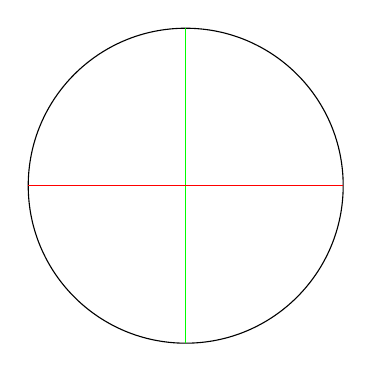
\begin{tikzpicture}
                \draw (0, 0) circle (2);
                \draw[red] (0, 0) -- (2, 0);
                \draw[green] (0, 0) -- (0, 2);
                \draw[red] (0, 0) -- (-2, 0);
                \draw[green] (0, 0) -- (0, -2);
            \end{tikzpicture}
        \end{center}

        Now consider the 3d space. $O = \{(l_1, l_2, l_3): l_1 \perp l_2, l_2 \perp l_3, l_1 \perp l_3\}$. Suppose for every triple in $O$, we paint one line red and the other two green. Can we paint every point in space red or green? 

        No! It is impossible. 
        
        \emph{Proof:} Let 
        \[L = \{\text{33 specifically chosen lines}\} \subset \{\text{the set of lines through the origin in } \R^3\}\]
        and 
        \[O = \{(l_1, l_2, l_3) : l_1, l_2, l_3 \in L, \; l_1 \perp l_2, l_2 \perp l_3, l_3 \perp l_1\}\]
        (Note that $\abs{O} = 16$). Finally, let $A = \{(1, 1, 0), (1,0,1), (0, 0, 1)\}$. Our problem thus reduces to showing that for this very particular subset of $\R^3$, $\not \exists m: O \to A$. 

    \subsection*{3 Spin States}
        \textbf{Basis:} We create a new basis for $\C_1^3$:
        \[\ket{u} = \begin{pmatrix}
            1\\0\\0
        \end{pmatrix}, \quad \ket{n} = \begin{pmatrix}
            0\\1\\0
        \end{pmatrix}, \quad \ket{d} = \begin{pmatrix}
            0\\0\\1
        \end{pmatrix}\]
        Such that any $\ket{\psi} \in \C_1^3$ can be written 
        \[\ket{\psi} = \alpha \ket{u} + \beta \ket n + \delta \ket{d}\]
        with $\abs \alpha^2 + \abs \beta^2 + \abs \delta^2 = 1$.

        \textbf{Measurements:} We define the spin operators by
        \[\sigma_z = \begin{pmatrix}
            1 & 0 & 0\\
            0 & 0 & 0\\
            0 & 0 & -1
        \end{pmatrix}, \quad \sigma_y = \frac{i}{\sqrt 2}\begin{pmatrix}
            0 & -1 & 0\\
            1 & 0 & -1\\
            0 & 1 & 0
        \end{pmatrix}, \quad \sigma_x = \frac{1}{\sqrt 2}\begin{pmatrix}
            0 & 1 & 0\\
            1 & 0 & 1\\
            0 & 1 & 0
        \end{pmatrix}\]
        
        \textbf{Expected values:} as before, 
        \[\E[\lambda_{\sigma_z}^2 \; | \; \ket{\psi}] = \E[\lambda_{\sigma^2_z} \; | \; \ket \psi] = 1^2 \abs{\brak{\psi \; | \; u}}^2 + 0^2 \abs{\brak{\psi \; | \; n}}^2 + (-1)^2 \abs{\brak{\psi \; | \; d}}^2\]
        (the coefficients are the eigenvalues of the operator so squaring just squares the eigenvalues).

        And by analogy, we get the mean squared spin states by $\sigma_x^2, \sigma_y^2, \sigma_z^2$: 
        \[\sigma_z^2 = \begin{pmatrix}
            1 & 0 & 0\\
            0 & 0 & 0\\
            0 & 0 & 1
        \end{pmatrix}, \quad \sigma_y^2 = \begin{pmatrix}
            \frac{1}{2} & 0 & -\frac{1}{2}\\
            0 & 1 & 0\\
            -\frac{1}{2} & 0 & \frac{1}{2}
        \end{pmatrix}, \quad \sigma_x^2 = \begin{pmatrix}
            \frac{1}{2} & 0 & \frac{1}{2}\\
            0 & 1 & 0\\
            \frac{1}{2} & 0 & \frac{1}{2}
        \end{pmatrix}\]

        This is very useful because while the spin operator matrices do not commute, the squared spin operator matrices do!
        \[[\sigma^2_x, \sigma^2_y] = [\sigma^2_x, \sigma^2_z] = [\sigma^2_y, \sigma^2_z] = 0\]s
        so there exists a common set of $3$ eigenvectors: 
        \[\ket{e_1} = \begin{pmatrix}
            0\\1\\0
        \end{pmatrix}, \quad \ket{e_2} = \begin{pmatrix}
            1/\sqrt 2\\0\\1/\sqrt 2
        \end{pmatrix}, \quad \ket{e_3} =  \begin{pmatrix}
            1/\sqrt 2\\0\\ -1/\sqrt 2
        \end{pmatrix}\]

        Which lets us create a table to read off the corresponding eigenvalues:
        \begin{center}
            \begin{tabular*}{1.28in}{|c|ccc|}
                \hline 
                & $\sigma_x^2$ & $\sigma_y^2$ & $\sigma_z^2$\\
                \hline
                $\ket{e_1}$ & $1$ & $1$ & $0$\\
                $\ket{e_2}$ & $1$ & $0$ & $1$\\
                $\ket{e_3}$ & $0$ & $1$ & $1$\\
                \hline
            \end{tabular*}
        \end{center}

        \textbf{Conclusion:} These are precisely the pairs in $A$! Results are not defined until they are measured. There does not exist a hidden $h$ such that $\forall l \in L$, $\lambda_l = l(h)$.

        This is precisely the same conclusion as we got from Bell's without using probabilities at all. 

\section*{Lecture 30: Nov 27}
    \subsection*{Background in $\C_1^3$}
        \textbf{A combinatorial result:}
        
        $L$ is a particular set of lines through the origin with $\abs{L} = 33$. $O$ is the set of triples of lines in $L$ which are mutually perpendicular. $A = \{(1, 1, 0), (1, 0, 1), (0, 1, 1)\}$. 

        \emph{Kochen-Specker Theorem:} There does not exist a function $m: L \to \{0, 1\}$ for which 
        \[(m(l_1), m(l_2), m(l_3)) \in A \qquad \forall (l_1, l_2, l_3) \in O\]

        \textbf{Spin 2 State Space:} We have basis vectors
        \[\ket{u} = \begin{pmatrix}
            1\\0\\0
        \end{pmatrix}, \quad \ket{n} = \begin{pmatrix}
            0\\1\\0
        \end{pmatrix}, \quad \ket{d} = \begin{pmatrix}
            0\\0\\1
        \end{pmatrix}\]
        leading to arbitrary states 
        \[\ket{\psi} = \alpha\ket u + \beta \ket n + \delta \ket{d} \in \C_1^3\]

        We can also calculate spin operators, 
        \[\sigma_x = \begin{pmatrix}
            0 & 1/\sqrt 2 & 0\\
            1/\sqrt 2 & 0 & 1/\sqrt 2\\
            0 & 1/\sqrt 2 & 0
        \end{pmatrix}, \quad \sigma_y = \begin{pmatrix}
            0 & -i/\sqrt 2 & 0\\
            i/\sqrt 2 & 0 & -i/\sqrt 2\\
            0 & i/\sqrt 2 & 0
        \end{pmatrix}, \quad \sigma_z = \begin{pmatrix}
            1 & 0 & 0\\
            0 & 0 & 0\\
            0 & 0 & -1
        \end{pmatrix}\]
        whose eigenvalues are all in $\{-1, 0, 1\}$ 

        We also have squared operators $\sigma_x^2, \sigma_y^2, \sigma_z^2$ which correspond to measuring $\lambda_x^2, \lambda_y^2, \lambda_z^2 \in \{0, 1\}$.

        As in the spin 1 case, these squared operators commute if and only if there exists a common set of eigenvectors: 
        \[\ket{e_1} = \begin{pmatrix}
            0\\1\\0
        \end{pmatrix}, \quad \ket{e_2} = \begin{pmatrix}
            1\\0\\1
        \end{pmatrix}, \quad \ket{e_3} = \begin{pmatrix}
            1\\0\\-1
        \end{pmatrix}\]

        Using these eigenvectors, we create a chart of eigenvalues for the squared operators:
        \begin{center}
            \begin{tabular*}{2in}{|c|ccc|}
                \hline 
                & $\sigma_x^2$ & $\sigma_y^2$ & $\sigma_z^2$\\
                \hline
                $\ket{e_1}$ & $1$ & $1$ & $0$\\
                $\ket{e_2}$ & $1$ & $0$ & $1$\\
                $\ket{e_3}$ & $0$ & $1$ & $1$\\
                \hline
            \end{tabular*}
        \end{center}

    \subsection*{The No-Go Theorem}
        Because of the Kochen-Specker Theorem and rotational invariance for all $(l_1, l_2, l_3) \in O$, we have a problem: If measurements could be known before hand (e.g. by knowing a hidden variable $h \in H$ a la Einstein's belief), then we could say the eigenvalues were functions of $h$ that took a value in $\{(1, 1, 0), (1, 0, 1), (0, 0, 1)\}$. But this is impossible!

        This is a \emph{stronger} result than Bell's Theorem because it does not make use of probability. So we have yet another no-go on hidden variables.

        \textbf{A way out:} There is still a way hidden variables could work though! Suppose $h \to h \times h_a$ for a particle $a$.

        Consider the singlet in $\C_1^3$:
        \[\ket{S} = \frac{1}{\sqrt 3}(\ket{ud} + \ket{nn} - \ket{du})\]

        For this state, we have six measurements that are very easy to calculate. Furthermore, they all commute with each other and share the same eigenvectors: 
        \begin{center}
            \begin{tabular*}{2in}{|c|cccccc|}
                \hline 
                & $\ket{e_1e_1}$ & $\ket{e_2e_2}$ & $\ket{e_3e_3}$\\
                $\sigma_x^2 \otimes I$ & $1$ & $1$ & $0$\\
                $\sigma_y^2 \otimes I$ & $1$ & $0$ & $1$\\
                $\sigma_z^2 \otimes I$ & $0$ & $1$ & $1$\\
                $I \otimes \sigma_x^2$ & $1$ & $1$ & $0$\\
                $I \otimes \sigma_y^2$ & $1$ & $0$ & $1$\\
                $I \otimes \sigma_z^2$ & $0$ & $1$ & $1$\\
                \hline
            \end{tabular*}
        \end{center}

        This leads to the \emph{TWIN} property: particle 2 is clearly a twin of particle 1.

        What if the particles are very far apart? Imagine the light cones from the two particles. If there is a hidden particle, then the state of $b$ depends on $h \times h_b$. But we can arrange the light cones so that $h_b$ is outside the light cone of $a$ and $h_a$ is outside the light cone of $b$. By special relativity, we can make it such that Bob chooses $h_b$ in Alice's future. Thus, Alice's choice of $h_a$ cannot depend on Bob's choice of $h_b$. But similarly, Alice chooses in Bob's future.

\section*{Lecture 31: Nov 29}
    \subsection*{Overview of Quantum Computing}
        \begin{enumerate}
            \item  We have a sequence of $n$ particles in energy wells. We can represent the state of the system as a vector in $\C^{2\otimes n} = \underbrace{\C_1^2 \otimes \C_1^2 \otimes \dots \otimes \C_1^2}_n$.
            \item Initialize $\ket{\psi_0} \in \C_1^{2\otimes n}$
            \item Perform a sequence of unitary operators with the goal of finding a $\ket{g} \in \C_1^{2\otimes n}$ such that $g \iff x \in \{0, 1\}^n$ ($x = x_1, x_2, \dots,\; x_n \in 2^n$)
            \item Iterate operators until $\ket{\psi_t} \approx \ket{g}$ (i.e. $\forall \varepsilon > 0: \P(\ket{\psi} \to \ket{g}) > 1 - \varepsilon$)
            \item Readout: measure $\ket{\psi}$ by measuring each coordinate (so that all measurements commute)
        \end{enumerate}
       
    \subsection*{Essential Background}
        \textbf{Unitary Operator:} $UU^\dagger = U^\dagger U = I$ (reflections and rotations)

        Every unitary operator $U$ can be realized (by a physical machine) 

        Evolution of a physical system is accomplished through unitary operators (because of preservation of total probability mass)
        \[\ket{\psi(t)} = U_t\ket{\psi_0} \implies \frac{d\psi}{dt} = -i\hbar H\ket{\psi(0)} \iff \ket{\psi(t)} = e^{-\frac{i}{\hbar}Ht}\ket{\psi(0)}\]

        And the spectral representation of unitary operators is given by 
        \[U = \sum_{k=1}^m e^{i\theta k}\ket{e_k}\bra{e_k}\]
        which implies a Hamiltonian operator with real values 
        \[H = \sum_{k=1}^m \theta_k \ket{e_k}\bra{e_k}\]

        \textbf{Conclusion:} for any unitary operator, we can find a Hamiltonian representing a real physical state/environment for which we can build a machine that will induce that state. Thus, we can build a machine that will perform any unitary operator by running long enough.

        \textbf{Notation:}
            \begin{itemize}
                \item $\ket{u} \leftrightarrow \ket{0}$
                \item $\ket{d} \leftrightarrow \ket{1}$
                \item $X = (X_1, \dots,\; X_n) \in \{0, 1\}^n \leftrightarrow \ket{x} \in \C_1^{2\otimes n}$ 
                \item $\ket{\psi} = \sum_{x_1, x_2, \dots,\; x_n} \gamma_{x_1, x_2, \dots,\; x_n}\ket{x_1, x_2, \dots,\; x_n} = \sum_x \gamma_x \ket{x}$ where $x$ is all sequence of $2^n$ zeros and ones 
            \end{itemize}

        \emph{Example:} 
        \begin{align*}
            \ket{\psi} &= (\frac{1}{\sqrt 2})^3 \sum_x \ket{x} \in \C_1^{(2 \otimes 3)}\\ 
                &= (\frac{1}{\sqrt{2}})^3 (\ket{uuu} + \ket{uud} + \ket{udu} + \ket{duu} + \ket{udd}  + \ket{dud} + \ket{ddu} + \ket{ddd})\\
                &= \ket{r} \otimes \ket{r} \otimes \ket{r}
        \end{align*} 

        In fact, this makes a very good initial state because it is ``neutral'' with respect to the up and down directions. 

        How do we measure $\ket{\psi}$? Say we have $\ket{\psi(T)}$ and we want to measure it. We know 
        \[\P(\ket{\psi} \to \ket{g}) > 1 - \varepsilon\]
        but in general, 
        \[\P(\ket{\psi} \to x) = \abs{\brak{x \; | \; \psi}}^2\]
        and 
        \[A \otimes B = (A \otimes I)(I \otimes B) = B \otimes A\]

\section*{Lecture 32: Dec 01}
    \subsection*{Quantum Computing}
        We have a data stucture called the \emph{register} 
        \[x = (x_1, x_2, \dots,\; x_n) \in \{0, 1\}^n \leftrightarrow \ket{x_1} \otimes \ket{x_2} \otimes \dots \otimes \ket{x_n} \in \C^{2 \otimes n}\]
        with $x_k = 1 \leftrightarrow \ket{d}, \quad x_k = 0 \leftrightarrow \ket{u}$

        \textbf{Basis:} $B = \{\ket{x}: (x_1, x_2, \dots,\; x_n) \in \{0, 1\}^{n}\}$ with 
        \[\ket{\psi} = \sum_{x_1} \sum_{x_2}\dots \sum_{x_n} \gamma_{x_1, \dots,\; x_n} \ket{x_1} \otimes \dots\otimes \ket{x_n} = \sum_{x\in B} \gamma_x \ket{x}\]

       \textbf{Generic operator:}
        \[\sum_{i=1}^m\gamma_{i} \gamma_i A_1 \otimes A_2 \otimes \dots \otimes A_n\]

        \emph{Example in $\C^2 \otimes \C^2$:} $A_1 \otimes B_1 + A_2 \otimes B_2$

        \textbf{Readout:} we measure each particle in the register independently using
        \[\sigma_{z_i} = \underbrace{I \otimes \dots \otimes I}_{i-1}\otimes \sigma_z \otimes \underbrace{I \otimes \dots \otimes I}_{n-i-1}\]

        And since for all $i$, the $\sigma_{z_i}$s commute, we can measure in any order. 

        \textbf{Goal (Boolean Satisfiability):} Given a boolean function $f: \{0, 1\}^n \to \{0, 1\}$, find $g \in \{0, 1\}^n$ such that $f(g) = 1$. We assume that there is a unique $g$ that satisfies this property. 

        The best known classical algorithm for this search problem is $O(2^n)$ (i.e. brute force).
        
        Grover's Algorithm does it in $O(2^{n/2})$.
        
        \emph{Boolean function Example (XOR/CNOT):} 
        \[\begin{cases}
            \{0, 1\} \to 1\\ 
            \{1, 0\} \to 1\\
            \{0, 0\} \to 0\\
            \{1, 1\} \to 0
        \end{cases} \longleftrightarrow \begin{pmatrix}
            1 & 0 & 0 & 0\\
            0 & 1 & 0 & 0\\
            0 & 0 & 0 & 1\\
            0 & 0 & 1 & 0
        \end{pmatrix}\]

    \subsection*{Grover's Algorithm}
        \begin{enumerate}
            \item \textbf{Prepare the register.} Notice that $(-1)^{f(x)}\ket{x}$ is a unitary operator on $\ket{x}$. Further, by uniqueness of $g$, 
            \[(-1)^{f(x)}\ket{x} = \begin{cases}
                -\ket{x} \qquad x = g\\
                \ket{x} \qquad x \neq g
            \end{cases}\]

            Because it is unitary, we can build a machine to create it via Schrodinger and the Hamiltonian. But also, we can prepare the register in such a way that all the elements are entangled which means that they are in a superposition of all possible states in the space -- one of which must be $g$. 

            Thus, we initialize the register 
            \[\ket{\psi'} = \frac{1}{\sqrt{2^n}} \sum_x \ket{x} = \frac{1}{\sqrt 2}\ket{r} \otimes \ket{r} \otimes \dots \otimes \ket{r}\]
            
        \end{enumerate}

\section*{Lecture 33: Dec 4}
    \subsection*{Setup}
        Let $f: \{0, 1\}^n \to \{0, 1\}$ be a boolean function with a unique $g$ such that $f(g) = 1$.
        
        We designate a basis by the set 
        \[\{\ket{x} = \ket{x_1, \dots,\; x_n} : (x_1, \dots,\; x_n) \in \{0, 1\}^n\}\]

        And let the state space be 
        \[V = \{\sum_{x = x_1}^{x_n} \gamma_x \ket{x} \bigg\vert \; \sum_x \abs{\gamma_x}^2 = 1\}\]

        And prepare the register of particles $x_1, \dots, x_n$ by 
        \[\ket{\psi} = \frac{1}{\sqrt{2^n}}\sum_x \ket{x} = \ket{r} \otimes \ket{r} \otimes \dots \otimes \ket{r}\]

        Suppose we are given an ``oracle'' which evaluates $f(x)$.

        Thus, we are searching the state space $\mathbb{V}$ for the input which the oracle evaluates to $1$.

        Lastly, we define 
        \[\ket{\psi'} = \frac{1}{\sqrt{2^{n}-1}}\sum_{x \neq g} \ket{x}\] 
        and a subspace 
        \[S = \{x\in \mathbb{V}: \ket{x} = \alpha \ket{g} + \beta \ket{\psi'},\; \alpha^2 + \beta^2 = 1, \; \alpha, \beta \in \R\}\]

        Notice that $\mathbb{V}$ is a space of dimension $2^n$ and $S$ is a linear space of two real dimensions.  
    \subsection*{The Process}
        Notice that
        \begin{enumerate}
            \item $\brak{g \; | \; \psi'} = 0$
            \item $\ket{g}, \ket{\psi}, \ket{\psi'}$ are all linear combinations of $\ket{g}$ and $\ket{\psi'}$ with real coefficients:
            \begin{align*}
                \ket{g} &= 1 \ket{g} + 0\ket{\psi'}\\ 
                \ket{\psi'} &= 0\ket{g} + 1\ket{\psi'}\\ 
                \ket{\psi} &= \frac{1}{2^n}\ket{g} + \frac{\sqrt{2^n -1}}{\sqrt{2^n}}\ket{\psi'}
            \end{align*}
        \end{enumerate}

        So $\ket{g}, \ket{\psi}, \ket{\psi'} \in S$. 

        We have a picture: 
        \usetikzlibrary{angles,quotes}
        \begin{center}
            \begin{tikzpicture}
                % Draw axes
                \draw[->] (0,0) -- (3,0) node[right] {$g$};
                \draw[->] (0,0) -- (0,3) node[above] {$\psi'$};
            
                % Draw line for y=3x
                \draw[domain=0:1, smooth, variable=\x, red, ->] plot ({\x}, {3*\x}) node[right] {$\psi$};
            
                % Draw dashed line from tip of y=3x to y-axis
                \draw[dashed] (1,3) -- (1,0);
            
                % Label angle with phi
                \coordinate (A) at (1,0);
                \coordinate (B) at (0,0);
                \coordinate (C) at (1,3);
                \pic[draw, angle radius=0.5cm, "$\phi$"] {angle = A--B--C};
            
                % Label distance on x-axis
                \node at (0.5, 0) [below, blue] {$\underbrace{\quad}_{\frac{1}{\sqrt{2^n}} \approx 0}$};
            \end{tikzpicture}
        \end{center}
        and since the distance is negligible, $\phi \approx \frac{\pi}{2}$

        Any unitary operator $U: S \to S$ will satisfy 
        \[U(\alpha\ket{g} + \beta\ket{\psi'}) = \alpha U\ket{g} + \beta U\ket{\psi'}\]
        so we can define $V$ by
        \begin{gather*}
            V = I - 2\ket{g}\bra{g}\\
            Vx = \begin{cases}
                -1 \quad x = g\\
                1 \quad\; x \neq g 
            \end{cases} = (-1)^{f(x)} \ket{x}
        \end{gather*}

        We can check that $V^\dagger V = VV^\dagger = I$ and add another operator 
        \[W = 2\ket{\psi}\bra{\psi} - I\]

        So $WV$ is unitary. Doing some arithmetic, we find
        \begin{align*}
            WV\ket{g} &= a\ket{g} - b\ket{\psi'}\\
            WV\ket{\psi'} &= b\ket{g} + a\ket{\psi'}
        \end{align*}
        and 
        \begin{align*}
            a &= (1 - \frac{2}{2^n})\\ 
            b &= \frac{2\sqrt{2^n - 1}}{2^n}
        \end{align*}
        which means that $WV$ acts on $S$ be a rotation clockwise through 
        \[\theta = \sin^{-1}(b) = \sin^{-1}(\frac{2\sqrt{2^n-1}}{2^n}) \approx \frac{1}{\sqrt{2^n}}\]

        Thus, by repeatedly applying $VW$ we can get arbitrarily close to $\theta = 0$ and thus find $g$. 

\section*{Lecture 34: Dec 06}
    \subsection*{Quantum Gates}
        In the implementation of Grover's Algorithm, we used two gates, $V$ and $W$, that seemed to be arbitrary. Here we will explore $V$ a bit more. 

        We'll use the usual basis $B = \{\ket{x_1, \dots,\; x_n} : x_k \in \{0, 1\}\}$ and a boolean function $f: \{0, 1\}^n \to \{0, 1\}$

        Recall from above that 
        \[V \ket{x} = (-1)^{f(x)}\ket{x} \quad \ket{x}\in B\]
        so the effect of $V\ket{\psi}$ is to act on the superposition of all possible states to ``mark'' the solution $g$ by changing the sign of the amplitude of $\ket{g}$: 
        \[V\ket{\psi} = V\sum_x \gamma_x \ket{x} = \sum_x \gamma_x V\ket{x} = \sum_x \gamma_x (-1)^{f(x)}\ket{x}\]

        Now we define a new operator $\oplus$ which takes $\ket{x, y} \to \ket{x, x \oplus y}$ where $x, y \in \{0, 1\}$ and $x \oplus y = x + y \mod 2$: 
        \begin{align*}
            (0, 0) \to (0, 0)\\ 
            (0, 1) \to (0, 1)\\ 
            (1, 0) \to (1, 1)\\ 
            (1, 1) \to (1, 0)
        \end{align*}
        which can be express as a matrix 
        \[\oplus = \begin{pmatrix}
            1 & 0 & 0 & 0\\ 
            0 & 1 & 0 & 0\\ 
            0 & 0 & 0 & 1\\ 
            0 & 0 & 1 & 0
        \end{pmatrix}\]
        and this happens to be precisely CNOT. 

        The problem is that if we applied this directly to $\ket{\psi}$, we would no longer have a unitary operator because some info was destroyed. To solve this, we add an \emph{ancillary bit} so $x \to \ket{x, y}$ so our oracle now looks like:
        \begin{center}
            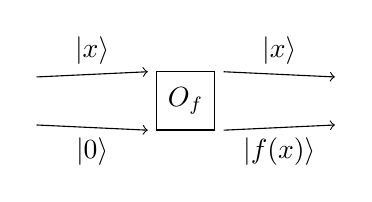
\begin{tikzpicture}
                \node[draw, minimum size=2.1em] (Of) at (0,0) {$O_f$};
                \draw[->, shorten >=3pt, shorten <=3pt] (-2,0.3) -- (Of.north west) node[midway, above] {$\ket{x}$};
                \draw[->, shorten >=3pt, shorten <=3pt] (-2,-0.3) -- (Of.south west) node[midway, below] {$\ket{0}$};
                \draw[->, shorten >=3pt, shorten <=3pt] (Of.north east) -- (2,0.3) node[midway, above] {$\ket{x}$};
                \draw[->, shorten >=3pt, shorten <=3pt] (Of.south east) -- (2,-0.3) node[midway, below] {$\ket{f(x)}$};
            \end{tikzpicture}
        \end{center}

        Now we have 
        \[H\ket{x} = \begin{pmatrix}
            1/\sqrt 2 & 1/\sqrt 2\\ 
            1/sqrt 2 & -1/\sqrt 2
        \end{pmatrix}\ket{x} \to \begin{cases}
            \ket{r} = \frac{1}{\sqrt 2}(\ket{o} + \ket{i}) \qquad x = 0\\ 
            \ket{l} = \frac{1}{\sqrt 2}(\ket{o} - \ket{i}) \qquad x = 1 
        \end{cases}\]

        Which gives us a full circuit, 
        \begin{center}
            \begin{tikzpicture}
                \node (x) at (0, 5) {$\ket{x}$};
                \node (o) at (0, 3) {$\ket{o}$};
                \node (i) at (0, 1) {$\ket{i}$};

                \draw (2, 2) rectangle ++(2, 4) node[midway]{$O_f$};

                \node (l) at (6, 1) {$\ket{l}$};
                \node (f) at (6, 3) {$\ket{f(x)}$};

                \draw (8, 0) rectangle ++(2, 4) node[midway]{$\oplus$};

                \node (x2) at (12, 5) {$\ket{x}$};
                \node (f2) at (12, 3) {$\ket{f(x)}$};
                \node (l2) at (14, 1) {$\begin{cases} 
                    -\ket{l} \quad \text{if } \ket{f(x)} = 1\\ 
                    \ket{l} \quad \text{if } \ket{f(x)} = 0
                \end{cases}$};
            
                \draw[->, shorten >=3pt, shorten <=3pt] (x) -- (2, 5);
                \draw[->, shorten >=3pt, shorten <=3pt] (o) -- (2, 3);
                \draw[->, shorten >=3pt, shorten <=3pt] (i) -- (l) node[midway, above] {$H$};
                \draw[->, shorten >=3pt, shorten <=3pt] (l) -- (8, 1);
                \draw[->, shorten >=3pt, shorten <=3pt] (4, 5) -- (x2);
                \draw[->, shorten >=3pt, shorten <=3pt] (4, 3) -- (f) -- (8, 3);
                \draw[->, shorten >=3pt, shorten <=3pt] (10, 1) -- (l2);
                \draw[->, shorten >=3pt, shorten <=3pt] (10, 3) -- (f2);                
            \end{tikzpicture}
        \end{center}

        So a single bit is flipped for the correct input and we can see that by measuring the outputted $\ket{x}$ 
\end{document} 
 